\documentclass{ucbthesis}
\usepackage[firstinits=true, uniquename=false, uniquelist=false, style=numeric-comp, maxcitenames=100, sortcites=true, natbib=true, block=space, url=false, doi=false, isbn=false, backend=biber]{biblatex}
\usepackage{textgreek}
% \usepackage{graphicx}
\usepackage[pdftex]{graphicx}
\usepackage{sidecap}
\usepackage{rotating}
\usepackage{caption}

\captionsetup[SCfigure]{labelformat=empty}

\def\changemargin#1#2{\list{}{\rightmargin#2\leftmargin#1}\item[]}
\let\endchangemargin=\endlist

% Double spacing, if you want it.
% \def\dsp{\def\baselinestretch{2.0}\large\normalsize}
% \dsp

% If the Grad. Division insists that the first paragraph of a section
% be indented (like the others), then include this line:
% \usepackage{indentfirst}

\newtheorem{theorem}{Jibberish}

\bibliography{references}

\hyphenation{mar-gin-al-ia}

\begin{document}

% Declarations for Front Matter

\title{Plasticity of neural circuits in the auditory system}
\author{Robert Roland Gibboni III}
\degreesemester{Fall}
\degreeyear{2014}
\degree{Doctor of Philosophy}
\chair{Professor Shaowen Bao}
\othermembers{Professor Yang Dan \\
  Professor Fr\a'ed\a'eric E. Theunissen \\
  Professor Michel Maharbiz}
\numberofmembers{4}
\prevdegrees{B.S. (University of Arizona) 2005}
\field{Neuroscience}
\campus{Berkeley}

% The title page generated by LaTeX is now acceptable for handing in.
% (This was not always the case).

\maketitle
% \approvalpage
\copyrightpage

\begin{abstract}
An understanding of plasticity, the ability of the brain to reorganize based on experience, is fundamental to understanding how the brain functions. Previous research has uncovered the molecular and cellular mechanisms by which neural activity leads to specific neural circuit modifications, but in order to appreciate their role in learning and memory, studies of large-scale neural systems are required. In this dissertation, I describe several studies that take advantage of mouse lines possessing mutations in genes known to be important for distinct types of plasticity.\\

% \vspace{.01in}
\noindent A mouse line lacking the \textit{Fmr1} gene replicates many of the disease phenotypes of Fragile X Syndrome (FXS), the most common single-gene determinant of mental disability in humans. \textit{Fmr1} knock-out (KO) mice do not undergo the critical period for auditory map plasticity, by which auditory cortex adapts to the sound milieu experienced immediately after hearing onset. Pharmacological blockade of group I metabolic glutamate receptors (mGluR) with 2-Methyl-6-(phenylethynyl)pyridine (MPEP) rescues this critical period, in agreement with the mGluR Theory of FXS.\\

% \vspace{.01in}
\noindent I also present work in a mouse that lacks tumor necrosis factor-\textalpha{} (TNF-\textalpha{}), which is critical for the expression of homeostatic regulation of synaptic strength. Auditory cortical development is disrupted in the TNF-\textalpha{} KO mouse, however auditory map expansion occurs normally. TNF-\textalpha{} is also required for \textit{in vivo} homeostatic regulation using a multi-frequency tone exposure paradigm. Early-life acoustic stimulation with multiple frequencies leads to a homeostatic decrease of spontaneous activity and narrowing of receptive field frequency bandwidths in wild-type animals, contrasted with KO animals, which experience an anti-homeostatic increase in spontaneous activity and broadening of receptive field bandwidths.\\

\noindent Finally, I describe a mouse model study of the role of homeostatic plasticity in tinnitus, a phantom sound percept that commonly accompanies partial hearing loss. The development of salicylate-induced and unilateral hearing loss-induced tinnitus-related behavior requires the presence of TNF-\textalpha{}. Direct application of recombinant TNF-\textalpha{} is sufficient to cause tinnitus-related behavior. In addition, reallocation of the deprived auditory cortex to ipsilateral ear inputs requires TNF-\textalpha{} expression. Single-gene knockout animals are valuable tools to extend our understanding of plasticity mechanisms from the molecular and cellular scale to the level of circuits and the intact brain.\\
\end{abstract}

\begin{frontmatter}

\begin{dedication}
\begin{center}
\vfil\null
My brain hurt like a warehouse\\
It had no room to spare\\
I had to cram so many things\\
To store everything in there\\
And all the fat-skinny people, and all the tall-short people\\
And all the nobody people, and all the somebody people\\
I never thought I'd need so many people\\
\vspace{5 mm}
---\textit{Five Years} by David Bowie\\
\vspace{30 mm}
To my family, friends, Haley Golden, and of course, Ponce de Le\'on\\
\end{center}
\end{dedication}

\tableofcontents
% \clearpage
% \listoffigures
% \clearpage
% \listoftables

\begin{acknowledgements}

\begin{quotation}
What would you do if I sang out of tune? Would you stand up and walk out on me?
\begin{flushright}
 ---Joe Cocker (Lennon/McCartney)
\end{flushright}
\end{quotation}


Graduate school is a funny thing. In a way, it is completely unlike anything I've ever seen or experienced. This idea is the primary force behind the popular conception of ``grad school"

as it is to refer to it as a postponement of joining the ``real world," The frontier of human knowledge is as bizarre and unpredictable. And like most frontiers, this one is best explored with some help.

\end{acknowledgements}

\end{frontmatter}

\pagestyle{headings}

\chapter{Introduction}

\section{Overview}

Plasticity, the ability to change, is a key feature of the brain's function. While much of development can be accomplished by unfurling genetically-encoded instructions, success is more likely when an individual can bring information from past experiences to bear on its response to new stimuli, i.e. when it can learn. The past century has seen enormous progress in the study of neural plasticity, from early conceptual models to specific molecular pathways. From these studies, we have learned of two main forms of plasticity that govern circuit modifications in the brain: Hebbian plasticity and homeostatic plasticity. Future advances will likely reveal how plasticity rules act and interact at the level of neural systems to generate the immense computational faculties of the brain.

\section{Early thoughts on plasticity}
The origins of a theoretical consideration of neural plasticity can be traced back to William James, who chose the term to refer to the changes that give rise to habitual behaviors \cite{James1910, Berlucchi2009}. Italian psychologists Eugenio Tanzi and Ernesto Lugaro and Spanish anatomist Santiago Ram\a`on y Cajal began to develop the idea that formation of new connections between neurons was the physiological instantiation of learning \cite{Berlucchi2009}. In his 1949 book, ``The Organization of Behavior," Donald Hebb clarified the idea of changing synaptic weights as a basis for learning. He described his model as follows \cite{Hebb1949}:

\begin{quotation}
Let us assume that the persistence or repetition of a reverberatory activity (or ``trace") tends to induce lasting cellular changes that add to its stability. [...] When an axon of cell A is near enough to excite a cell B and repeatedly or persistently takes part in firing it, some growth process or metabolic change takes place in one or both cells such that A's efficiency, as one of the cells firing B, is increased.
\end{quotation}

Hebb's rule, as this mechanism came to be known, charted new territory in the understanding of brain plasticity. It brought the field closer to the goal of a specific theory for how activity in a neural circuit is translated into instructions to modify that circuit to incorporate new information.

\section{From theory to physiology}

In 1968, Timothy Bliss and Terje L\o mo discovered experimental evidence for Hebbian plasticity in rabbit dentate granule cells \cite{Bliss1973}. They observed that high-frequency electrical stimulation of the perforant path inputs onto granule cells led to those inputs being strengthened. The finding closely matched the idea of a brain that operated according to Hebb's rule---strong electrical stimulation caused the pre-synaptic neurons to fire and drive activity in the post-synaptic neurons, leading to increased synaptic weights. This implementation of Hebbian learning, which has since been replicated in countless experiments, came to be known as ``long-term potentiation" or LTP, and serves as a foundation for how we understand neural plasticity to work.

Networks whose plasticity is governed solely by Hebbian plasticity are prone to unstable behavior. If a given synapse participates in driving the post-synaptic target to fire, its weight will be increased, causing it to be more likely to activate the post-synaptic neuron, increasing its weight, and so on. Conversely, a synapse that rarely activates the post-synaptic neuron will fall into a negative feedback loop and its weight will be reduced to zero. Not only is this an unusable learning process from a theoretical standpoint, it does not agree with experimental evidence showing the distribution of synaptic weights on a neuron to be normally distributed with a slight positive skew rather than the ``all-or-none" distibution predicted by purely Hebbian learning mechanisms \cite{Turrigiano1998}. Although Hebb described a powerful learning rule that appeared to actually operate in the brain, its instability in isolation led scientists to the hypothesis that there must be additional mechanisms at play that could ensure network stability.

That key missing component was a way to achieve activity \textit{homeostasis}, the preservation of activity (usually represented by neuronal firing rate) within a set range. An extraordinary number of factors determine the overall electrical activity of a neuron, and the brain seems to have evolved ways to modulate many of them to maintain homeostasis. The sodium, potassium, and calcium channels that determine a neuron's intrinsic excitability could be modulated \cite{Franklin1992}. The system could attenuate the degree of plasticity for strong synapses, preventing run-away synaptic strengthening \cite{VanRossum2000}. Another option is to increase or decrease the strengths of all synaptic inputs to the neuron to counteract deviations from the desired activity range. By multiplicatively scaling all synapses, the cell can change its overall activity level without sacrificing the information contained in the synaptic weights. This process is known as synaptic scaling, and itself appears to have several distinct mechanisms, as will be discussed later.

With the theoretical foundations in place and the physiological mechanisms outlined, a major challenge is to understand how these plasticity rules defined at the level of pairs of neurons or small neural assemblies operate and co\"operate to affect larger scale network dynamics and, finally, behavior. The current work aims to address this question using two mouse lines deficient in important molecular components of plasticity, Fragile X mental retardation protein (FMRP) and tumor necrosis factor-\textalpha{} (TNF-\textalpha{}).

\section{\textit{Fmr1} and plasticity}

Fragile X Syndrome (FXS) is the most common cause of inherited mental retardation, resulting from the transcriptional silencing of the \textit{Fmr1} gene and the absence of its protein product, fragile X mental retardation protein (FMRP) \cite{Bailey1998, Jin2003}. Mice lacking \textit{Fmr1} display many of the same disease phenotypes as humans with Fragile X Syndrome including learning deficits, hyperactivity, auditory hypersensitivity, social impairments, and macro\"orchidism \cite{DutchBelgianFragileXConsortium1994, Bernardet2006, Moy2008}, allowing scientists a better opportunity to uncover the physiological basis of the disease.

One common neuroanatomical finding in FXS is an increased density of thin, under-developed dendritic spines \cite{Hinton1991, Comery1997, Dolen2007, Liu2011} (although some recent studies call into question whether increased spine density is a reliable pathology \cite{Cruz-Martin2010, Harlow2010a, Meredith2007}). The advent of \textit{in vivo} optical imaging of spines revealed that a hallmark of \textit{Fmr1} knock-out (KO) neurons is that their dendritic spines have increased motility and turn-over \cite{Cruz-Martin2010, Pan2010}. This observation suggests an inability for networks lacking FMRP to stabilize synaptic connections, and could imaginably explain the processing deficits seen in FXS.

FMRP performs an impressive number of roles in the cell, many of them related to the translation of dendritic mRNAs that facilitates rapid, activity-dependent synaptic alteration. One study found that FMRP associates with 432 unique mRNAs, hinting at its important regulatory role \cite{Brown2001}. Not surprisingly given its promiscuity in the cell, there are direct links between \textit{Fmr1} and several specific plasticity mechanisms. Metabolic glutamate receptor (mGluR)-dependent LTD is enhanced in the hippocampus, although it is normal in cortex \cite{Huber2002}. Conversely, mGluR-dependent LTP is strongly attenuated in cortex, while it is normal in the hippocampus \cite{Li2002, Zhao2005, Wilson2007}. These deficits in synaptic plasticity could underlie some of the developmental abnormalities in FXS, for example the critical period for ocular dominance, which is absent in \textit{Fmr1} KO animals \cite{Dolen2007}.

FMRP also plays a role in retanoic acid-mediated synaptic scaling resulting from action potential and NMDAR blockade \cite{Soden2010}. This form of synaptic scaling is independent of protein transcription, but instead proceeds through translation of locally-available mRNAs for GluR1-type AMPA receptors that are then inserted into the post-synaptic membrane. Interestingly, FMRP does not appear to be required for synaptic scaling when NMDARs are left unobstructed, highlighting the fact that the brain employs redundant mechanisms to enforce homeostasis \cite{Soden2010}.

A major conceptual advance our understanding of \textit{Fmr1} and FXS came in 2004, when Bear, Huber, and Warren put forth a theory for FXS based on its interactions with mGluR. In wild-type cells, FMRP responds to mGluR5 activation by inhibiting mRNA translation in the synapse, effectively acting as negative feedback for the mGluR5 signaling pathway. Lacking FMRP, synaptic proteins are translated in excess, leading to undesirable consequences, including exaggerated long-term depression \cite{Huber2002, Bear2004}. Attenuation of mGluR signaling in mice reverses many of the abnormal phenotypes of FXS including spine morphology, impaired synaptic plasticity, protein overabundance, behavioral abnormalities, and the impaired critical period for ocular dominance \cite{DeVrij2008, Dolen2007, Su2011}.

\section{TNF-\textalpha{} and plasticity}

Tumor necrosis factor-\textalpha{} (TNF-\textalpha{}) is a protein traditionally regarded as a component of the pro-inflammatory response. It has recently been discovered to have a much wider range of effects, including an important role in proper neural function. In 2006, Stellwagen and Malenka discovered that synaptic scaling depends on the presence of glial TNF-\textalpha{}. Importantly, the absence of TNF-\textalpha{} had no effect on LTP and LTD, showing that the mechanisms for Hebbian and homeostatic plasticity do not significantly overlap and allowing future studies to consider the two processes with some degree of isolation \cite{Stellwagen2006}. The development of a mouse line lacking TNF-\textalpha{} gave researchers the ability to study the role of homeostatic plasticity in a wide range of \textit{in vivo} preparations.

This experimental tool led to a deeper understanding of a classic model for critical period plasticity, monocular deprivation-induced shift of ocular dominance. Occluding vision in one eye early in life leads to well-characterized changes to the cells in visual cortex receiving synaptic input from both eyes. First, synaptic connections from the deprived eye become weaker, then connections from the spared eye become stronger \cite{Frenkel2004}. The two phases of ocular dominance plasticity seem to be mediated by two specific plasticity mechanisms. Loss of connections from the deprived eye results from Hebbian LTD---noisy input from the blocked eye is no longer able to reliably fire the post-synaptic neuron, causing those synapses to be weakened. The increase in the synaptic strengths for spared eye inputs results from synaptic scaling---the overall lower synaptic drive leads to a reduction in firing rate for the post-synaptic neuron and the remaining synapses are up-scaled to bring activity back within the set range. In TNF-\textalpha{} mice, which lack the ability to scale up their synapses, deprived eye responses are lost, but spared eye responses never increase \cite{Kaneko2008}.

Although it is clear that TNF-\textalpha{} is necessary to express synaptic scaling, the precise relationship between TNF-\textalpha{} and homeostatic plasticity is complex and still unclear. A simple model in which decreasing activity leads to slowly accumulating release of TNF-\textalpha{} that signals insertion of additional AMPARs conflicts with the data. Instead, the effect of TNF-\textalpha{} appears to be state-dependent, leading to increases in synaptic strength when applied alone, and leading to decreases in synaptic strength when applied to prescaled synapses \cite{Steinmetz2010}. Thus, TNF-\textalpha{} does not directly signal synaptic scaling, but appears to play a permissive role, maintaining the neuron's ability to scale up synapses in the face of activity blockade \cite{Steinmetz2010}.

\section{Auditory cortical map plasticity}

Throughout the animal kingdom and throughout the brain, early experiences can exert profound and permanent influence on neural circuits. While learning can take place throughout life, in many neural systems there exists a restricted time interval during which stimuli can most readily alter the structure of the underlying network. One well-studied critical period regulates allocation of neural resources in the cortical auditory map. Sound processing in the brain begins in the cochlea, a complex spiral-shaped transduction apparatus in the inner ear. The receptors themselves, known as hair cells for the minute mechanosensory hairs they possess, are embedded in the basilar membrane, which coils along the core of the cochlea. The mechanics of the cochlea's physical structure decomposes pressure variations in the air, so that different frequency sound inputs displace hair cells at different locations along the basilar membrane. The result is a map of sound frequency. The orderly arrangement of frequency representations in space is known as tonotopy and is the most obvious feature of sound processing throughout the brain. Tonotopy is preserved all along the auditory pathway including primary auditory cortex (AI), where low frequency sounds activate neurons in caudal areas and high frequency sounds activate neurons in rostral areas.

The specific allocation of cortical area to different frequencies is determined during an early critical period. In rats, exposure to a 7-kHz tone between post-natal days (P) 11 and 14 leads to a significant increase in the percent of AI representing that tone. Importantly, the change persists many weeks after cessation of tone exposure, and the same exposure either before or after the P11-14 window does not lead to any significant changes to the tonotopic map \cite{DeVillers-Sidani2007}. Recent work is starting to shed light on the mechanisms underlying this critical period. Inhibitory circuits appear to play a crucial role. Around hearing onset, inhibitory currents are weak and are not co-tuned with excitation, as they are in the adult auditory cortex \cite{Dorrn2010}. In this state, pulsed tone presentation can lead to rapid alterations in the frequency tuning of neurons, and in addition, this susceptibility is lost with the appearance of closely matched excitation and inhibition. Additional support for the importance of inhibition comes from manipulations that postpone critical period closure, such as rearing in broadband noise, that also delay the normal time course of inhibitory maturation \cite{DeVillers-Sidani2008}. Why the presence of balanced excitation and inhibition in a network should render it invulnerable to alteration by experience is not yet clear, but it is a promising direction in advancing our understanding critical periods.

\section{Summary of present work}

In the current work, I describe the use of several experimental techniques including single-gene knockout organisms, intracortical injection of recombinant protein, behavioral assays, and multi-unit recording of cortical neural activity to understand the role of two key molecular players in neural plasticity, Fragile X mental retardation protein (FMRP) and tumor necrosis factor-\textalpha{} (TNF-\textalpha{}).

In Chapter 2, I present an experiment exploring the role of \textit{Fmr1} in the critical period for tonotopic map development. The study finds that in the absence of \textit{Fmr1}, the auditory map develops normally, however experience-induced map expansion does not occur. Treatment with MPEP, a drug targeted to correct the over-active mGluR pathway, restores normal critical period plasticity.

In Chapter 3, I describe development of the auditory map in mice lacking TNF-\textalpha{}. Tonotopic map development is impaired in a sound environment that is not specifically enriched with patterned sound. Early exposure to a pulsed pure tone leads to normal map expansion, indicating that the mechanisms underlying this critical period are intact in the TNF-\textalpha{} KO mouse.

In Chapter 4, I turn to the study of tinnitus, the perception of phantom sounds. First, I show that TNF-\textalpha{} KO mice do not show tinnitus-related behaviors following noise-induced hearing loss or salicylate treatment. I then show that intracortical injection of recombinant TNF-\textalpha{} is sufficient to cause tinnitus-related behavior in wild-type and knockout animals. I also describe the bilateral remapping of sound inputs to cortex following unilateral hearing lesion, and show that the rerouting of the intact ipsilateral input does not occur in mice lacking TNF-\textalpha{}.

\printbibliography
\chapter{Critical period plasticity in fragile X mice}

\section{Overview}
\newrefsection

Fragile X syndrome, the most common form of heritable mental retardation, is a developmental disorder with known effects within sensory systems. Altered developmental plasticity has been reported in the visual and somatosensory systems in \textit{Fmr1} knock-out (KO) mice. Behavioral studies have revealed maladaptive auditory responses in fragile X syndrome patients and \textit{Fmr1} KO mice, suggesting that adaptive plasticity may also be impaired in the auditory system. Here we show that, whereas tonotopic frequency representation develops normally in \textit{Fmr1} KO mice, developmental plasticity in primary auditory cortex is grossly impaired. This deficit can be rescued by pharmacological blockade of mGluR5 receptors. These results support the mGluR hypothesis of fragile X mental retardation and suggest that deficient developmental plasticity may contribute to maladaptive auditory processing in fragile X syndrome.

\section{Introduction}

Fragile X syndrome is caused by expansion of trinucleotide CGG repeats in the \textit{Fmr1} gene resulting in hypermethylation and loss of function of the gene (\cite{Jin2003}). \textit{Fmr1} encodes fragile X mental retardation protein (FMRP), an mRNA-binding protein that suppresses and regulates local mRNA translation. The lack of FMRP exaggerates mGluR-stimulated protein synthesis, which has been hypothesized to cause various fragile X symptoms (\cite{Bear2004, Osterweil2010}). Supporting this mGluR hypothesis of fragile X syndrome, the blockade of mGluR either genetically or pharmacologically reverses certain fragile X phenotypes in animal models (\cite{McBride2005, Yan2005, Dolen2007, DeVrij2008, Meredith2011, Su2011, Michalon2012, Thomas2012}).

Fragile X mental retardation is the most common form of heritable mental retardation. Among its symptoms are maladaptive sensory responses and impaired sensory integration (\cite{Miller1999, Chen2001, Nielsen2002}), which have been hypothesized to contribute to the impaired development of higher cognitive functions (\cite{Hanson1986, Leblanc2011}). Studies in mouse models lacking the \textit{Fmr1} gene revealed altered ocular dominance plasticity in visual cortex and a delayed critical period of synaptic plasticity in barrel cortex (\cite{Dolen2007, Harlow2010}). Altered auditory processing in humans with fragile X syndrome and \textit{Fmr1} knock-out (KO) animals suggests that development and plasticity in the auditory system may also be affected by fragile X syndrome (\cite{Miller1999, Chen2001, Nielsen2002}).

The development of acoustic representations in primary auditory cortex is profoundly influenced by early experience (\cite{Zhang2001, DeVillers-Sidani2007, Insanally2009, Popescu2010}). Exposure of juvenile animals to patterned sensory input refines the balance of excitation and inhibition (\cite{Dorrn2010, Sun2010}), resulting in receptive field and sensory map reorganization and a long-lasting impact on sound perception (\cite{Han2007}). The robust effects of early experience on sound representation and perception make the auditory cortex an ideal system to investigate how genetic mutations may lead to sensory abnormalities, such as those caused by fragile X mental retardation and \textit{Fmr1} gene deletion. In addition, cellular and synaptic abnormalities have been well characterized in the \textit{Fmr1} KO mouse, making it a valuable model to study the mechanisms of sensory development and plasticity.

In the present study, we investigate the development of cortical sound representations and sound-induced cortical map reorganization in the \textit{Fmr1} KO mouse. Our results indicate that the \textit{Fmr1} KO mouse develops a normal tonotopic cortical frequency map, but does not show experience-dependent map reorganization. Systemic administration of MPEP, an mGluR5 antagonist, rescues the impairment in cortical map plasticity.

\section{Methods}

\subsection{Rearing and injection procedures}

All procedures used in this study were approved by the Animal Care and Use Committee at the University of California, Berkeley. Wild-type (WT) and \textit{Fmr1} KO mice on the FVB background were originally obtained from The Jackson Laboratory (FVB.129P2-Pde6b+ Tyrc-ch/AntJ and FVB.129P2-Pde6b+ Tyrc-ch \textit{Fmr1}tm1Cgr/J). Only male homozygous WT or KO mice were used in this study. Litters of mouse pups were placed in sound-attenuating chambers with their mothers from postnatal day 9 (P9) through P20 (early window) and exposed to 16 kHz pure tone pips (25 ms duration, 60 dB) presented in trains of 6 pips (each train every 2 s and pips presented at 5 pips per second within a train) through an overhead speaker. Additional juvenile mice were exposed to the same sound stimuli at a later time window (P20-P30). Animals reared in a normal laboratory husbandry setting served as na\"ive controls.

Additional litters of animals, exposed to the same sound stimuli during either the early (P9-P20) or the late window (P20-P30), were also given daily injections of 2-methyl-6-(phenylethynyl)-pyrydine (MPEP; reconstituted to 2 mg/ml, injected at 30 mg/kg, i.p.; Sigma-Aldrich) or vehicle saline (15 ml/kg, i.p.). The weights of these animals were monitored daily to ensure proper development. Consistent with previous reports (\cite{Moy2009}), KO animals generally had larger body mass than WT animals. Sound exposure tended to reduce weight gain of KO animals and increase weight gain of WT animals (Table 1).

\centerline{\includegraphics[width=6in]{images/C2T1}}

\begin{changemargin}{1in}{1in}
\footnotesize{Table 1. AI size, threshold, peak latency, bandwidth at 50 dB, body mass, and number of animals used in all conditions. SEM is shown in parentheses. Two $\times$ 7 ANOVAs (genotype $\times$ condition) showed significant effects for overallsize, latency, and body mass. Significant main effects for condition were found for overall size of AI (**$p<0.005$) and latency (*$p<0.05$), but not for genotype or interaction. Significant main effects for genotype ($p<0.005$) and condition ($p<0.005$), and a significant interaction ($p<0.001$) were found for body mass.}
\end{changemargin}

After sound exposure, experimental animals were returned to a normal laboratory husbandry setting until the electrophysiological mapping of primary auditory cortex (typically P35-P45). A subset of early window exposure animals were recorded immediately after removal from the sound exposure box (P20-P25). Care was taken to ensure that all conditions (genotype, exposure condition, injection schedule) were age-matched during mapping, except the subset of animals that were mapped immediately after removal from the sound exposure box. Across the 16 conditions, a total of 76 animals were used for cortical electrophysiological experiments (Table 1). An additional 16 animals were used for auditory brainstem responses (ABRs).

\subsection{Electrophysiological recording procedure}

The primary auditory cortex (AI) of mice was mapped as previously described (\cite{Kim2009}), except as follows. Mice were anesthetized with ketamine (100 mg/kg, i.p.) and xylazine (10 mg/kg, i.p.), and supplemented as needed (ketamine 50 mg/kg, xylazine 5 mg/kg, i.p. generally once an hour). The cortex was maintained under a layer of silicone oil, reapplied as necessary. Multiunit responses to 25 ms pure tone pips (2-74 or 4-74 kHz, 0.1 octave increments at 0-70 dB, 10 dB increments) were recorded using tungsten microelectrodes (FHC) in the thalamorecipient layer of AI (350-450 micrometers below the cortical surface). References to neurons in this text refer to multiunit responses recorded extracellularly. Tones were presented to the left ear through an electrostatic speaker (Tucker Davis Technologies) at 3 pips per second and each frequency-intensity combination was repeated three times. Cortical penetration locations were recorded on a high-resolution image.

ABRs were recorded under identical anesthetic conditions with the active electrode at the vertex, the reference electrode caudomedial to the left ear pinna, and the ground electrode at the dorsosacrum (\cite{OConnor1998, Popescu2010}). Tone pips (4, 8, 16, and 32 kHz at 0-70 dB SPL in 5 dB increments) were presented to the left ear and ABRs were recorded ipsilaterally. Responses to 500 pips were averaged and high-pass filtered with a cutoff frequency of 200 Hz.

\subsection{Data analysis}

Receptive fields and response properties were isolated using custom-made programs in MATLAB as previously described (\cite{Insanally2010}), except as follows. The peak of the peristimulus time histogram (PSTH) within a window from 7 to 50 ms after the stimulus onset was defined as the response latency. The response window was defined as a period encompassing the PSTH peak, in which the firing rate was higher than the baseline firing rate. The spikes in the response window were counted to reconstruct the receptive field. The characteristic frequency (CF) and threshold of the receptive fields were identified by hand by a blind experimenter. Bandwidth at 50 dB was automatically calculated as previously described (\cite{Insanally2010}).

ABR thresholds at each frequency were determined as the lowest intensity that produced a visibly discernible response. Wave latency times were manually labeled for two frequency (8 and 16 kHz) and two intensity levels (70 and 45 dB). Wave amplitudes were calculated as the amplitude from a peak to an ensuing trough.

All error bars indicate SEM. Statistical tests are indicated in the text.

\section{Results}

\subsection{\textit{Fmr1} KO mice exhibit impaired critical period sensory map plasticity}

Litters of WT and KO animals were exposed to 16 kHz tones from P9 to P20. This window encompasses the critical period for frequency representation in rats (\cite{DeVillers-Sidani2007, Insanally2009}) and has been shown to elicit map plasticity in mice (\cite{Barkat2011}). Na\"ive WT and KO animals had very similar cortical frequency representation (Fig. 1A,B), suggesting normal auditory cortex development in KO mice. WT animals exposed to 16 kHz tone showed a substantial increase in representation of 16 kHz, whereas KO animals exposed to the same tone did not (Fig. 1A,B). A 2 × 2 × 10 ANOVA (genotype × exposure conditions × frequency bin) revealed a significant three-way interaction ($p=0.0009$), suggesting a differential representation to specific frequency bins between genotype and rearing condition. A further two-way ANOVA (genotype × exposure condition) on individual frequency bins found significant effects at 16 kHz (exposure condition, $p=0.00029$; genotype, $p=0.055$; interaction $p=0.024$; Fig. 1B), indicating representation of the exposed frequency increased in the WT mice only. The sound exposure had opposite effects on the representation of 21.11 kHz for the two genotypes (two-way ANOVA interaction, $p=0.0002$), reducing 21.11 kHz representation in the WT but not KO mice. Similar reduction of representations for frequencies near the exposure frequency has been previously reported (\cite{Han2007}).

\centerline{\includegraphics[height=4in]{images/C2F1}}

\begin{changemargin}{1in}{1in}
\footnotesize{Figure 1. \textit{Fmr1} KO mice exhibit impaired critical period plasticity in the auditory cortex. (A) Example AI frequency maps of two genotypes (WT and \textit{Fmr1} KO) and three conditions (na\"ive, early tone exposure, late tone exposure). Areas outlined in black indicate sites with CFs near the exposure frequency of 16 kHz ($\pm0.2$ octaves). Example receptive fields are shown for each map, with the location indicated by white roman numerals (x-axis is frequency from 2-74 kHz; y-axis is sound level from 0 to 70 dB). Scale bar, 1 mm. (B) Size of frequency representation for the na\"ive and early tone exposure groups. The WT early tone exposure group shows a significant increase in representation of 16 kHz (**condition main effect $p=0.00029$ and interaction $p=0.024$). A small decrease is also observed at 21.1 kHz (*interaction $p=0.0002$). (C) Representation of 16 kHz across four conditions (same as (A) with the addition of early tone exposure animals mapped immediately after removal from tone exposure box). Early tone exposure resulted in a significant increase in 16 kHz representation in the WT animals in both mapping windows (one-way ANOVA main effect $p<0.0005$, post hoc tests: *$p<0.05$ and **$p<0.005$). Sound exposure did not cause map changes in KO animals (one-way ANOVA, $p=0.13$).}
\end{changemargin}


\textit{Fmr1} KO mice exhibit impaired critical period plasticity in the auditory cortex. A, Example AI frequency maps of two genotypes (WT and \textit{Fmr1} KO) and three conditions (na\"ive, early tone exposure, late tone exposure). Areas outlined in black indicate sites...

This impairment in plasticity could be due to a delay in the critical period (\cite{Harlow2010}). To address this possibility, additional litters of animals were exposed to 16 kHz between P20 and P30. A 2 × 3 ANOVA [genotype × exposure condition (na\"ive, early exposure, late exposure)] revealed a significant main effect for exposure condition ($p=0.0001$) and a significant interaction ($p=0.015$). We find that only the WT mice that were sound exposed in the early window, but not the late window, had enlarged representation of 16 kHz (Fig. 1C). Neither the WT nor the KO mice that were sound-exposed in the late window showed enhanced representations of 16 kHz. Thus, the critical period for frequency-representation in mice does not extend beyond P20, and KO mice do not have a delayed critical period.

The lack of exposure-induced frequency map reorganization in the KO mice could also be due to previously reported hyperplasticity (\cite{Dolen2007}), which might have allowed a rapid reversal of the altered frequency map during the period of normal sensory experience before the auditory cortex was mapped. To address this possibility, additional litters of animals (WT: n = 4; KO: n = 6) were exposed to 16 kHz continually from P9 until the day of AI mapping (P20-P25; Fig. 1C). A one-way ANOVA comparing 16 kHz representation in na\"ive, early exposure, and early exposure immediately mapped WT animals reveal a significant effect ($p=0.0022$), with post hoc analyses showing no significant differences between the two early exposure groups that were mapped at different ages. A similar ANOVA on the KO animals shows a nonsignificant effect ($p=0.135$). Although the immediately mapped KO animals appear to show a slight increase in representation of 16 kHz, even an uncorrected comparison of the KO na\"ive and immediately mapped animals did not show a significant effect ($p=0.0988$).

\subsection{Auditory brainstem response differences are not frequency specific}

\textit{Fmr1} KO animals are impaired in experience-dependent regulation of potassium channels in the auditory brainstem (\cite{Strumbos2010}). To investigate potential subcortical plasticity, we compared ABRs between WT and KO mice that were either na\"ive or 16 kHz-exposed (P9-P20; Fig. 2A). Sound exposure reduced the ABR amplitude in WT mice and increased the amplitude in KO mice (genotype × exposure × frequency × intensity repeated measures four-way ANOVA: genotype effect, $p=0.038$; exposure, $p=0.0069$; their interaction, $p<0.0001$; Fig. 2B). However, this effect does not appear to be frequency specific, as the frequency interactions with genotype ($p=0.53$) and exposure ($p=0.41$) are not significant. The ABR threshold was not different between the genotypes and was not altered by sound exposure (ANCOVA on genotype × exposure with frequency as a covariate: genotype, $p=0.587$; exposure, $p=0.909$; interaction, $p=0.0609$; Fig. 2C).

\centerline{\includegraphics[width=4in]{images/C2F2}}

\begin{changemargin}{1in}{1in}
\footnotesize{Figure 2. ABRs are altered in \textit{Fmr1} KO mice, but not in a frequency-specific manner. (A) Example ABR traces recorded from WT and KO animals that were either na\"ive (NV, left) or 16 kHz-exposed (EXP, right). Responses were activated by 16 kHz tone pips. (B) Amplitudes of the five ABR waves recorded with 16 kHz tone pips at 70 dB. Sound exposure had different effects on WT and KO mice, increasing ABR amplitudes in KOs and reducing ABR amplitudes in WTs (genotype $\times$ exposure interaction, $p<0.0001$). (C) The ABR threshold was not different between the genotypes and was not altered by sound exposure. (D) Latencies of wave I (left) and wave IV (right). Latency for wave I was shorter for KOs than WTs ($p=0.0073$) and was not altered by sound exposure. Latency for wave IV was shortened by sound exposure in WTs, but delayed in KOs (genotype $\times$ exposure interaction, $p<0.001$). These effects were consistent across frequency (8 and 16 kHz) and sound level (45 and 70 dB).}
\end{changemargin}

ABRs are altered in \textit{Fmr1} KO mice, but not in a frequency-specific manner. A, Example ABR traces recorded from WT and KO animals that were either na\"ive (NV, left) or 16 kHz-exposed (EXP, right). Responses were activated by 16 kHz tone pips. B, Amplitudes ...

ABR latency was analyzed with two-way ANOVAs (genotype × exposure condition) for each discernible wave. In wave I, which represents early responses in the auditory nerve, KO mice had shorter latencies than WT mice and this difference was not altered by experience (genotype, $p=0.0073$; sound exposure,$p=0.87$; interaction, $p=0.55$; Fig. 2D). No significant effects were found for wave II or wave III, which represent responses from the spiral ganglion and cochlear nucleus, respectively (data not shown). Sound exposure reduced latencies in the WT groups, but increased them in the KO groups for waves IV and V, which represent responses from the superior olivary complex and inferior colliculus, respectively (interaction, $p<0.001$ and $p=0.006$, respectively; Fig. 2D). These effects were consistently seen for both the exposed (16 kHz) and nonexposed (8 kHz) frequencies, and at 45 and 70 dB sound pressure levels (Fig. 2D). These results indicate that, although FMRP deficiency and sound exposure significantly impacted ABRs, the effects are frequency-nonspecific and therefore cannot account for frequency-specific map reorganization in AI. Furthermore, the ABRs in the KO mice are not grossly impaired, and the ABR differences probably do not account for the impairment in auditory map plasticity.

\subsection{Daily injection of MPEP rescues plasticity deficit in KO mice}

It has been suggested that fragile X phenotypes are related to overactive Group 1 metabotropic glutamate receptors (\cite{Bear2004}). Indeed, genetic manipulations to suppress mGluR5 have been shown to rescue many fragile X phenotypes (\cite{Dolen2007}). In addition, pharmacological suppression of mGluR5 using MPEP or CTEP has been shown to correct many deficits in both mouse and Drosophila melanogaster models of fragile X syndrome (\cite{McBride2005, Yan2005, DeVrij2008, Meredith2011, Su2011, Michalon2012, Thomas2012}).

To investigate the role of mGluR in auditory critical period plasticity, we exposed additional litters of mice to 16 kHz during either the early (P9-P20) or late (P20-P30) window and systemically administered either MPEP or vehicle saline to littermates daily. We found that both MPEP- and saline-injected WT animals had larger representations of 16 kHz than na\"ive WT animals when they were exposed in the early window, but not the late window (Fig. 3A). A one-way ANOVA on the WT animals across the five conditions revealed a significant effect ($p=0.023$), with the early window saline and MPEP groups having significantly larger 16 kHz representations than the na\"ive groups [$p<0.05$ and $p<0.005$, respectively; Fig. 3B; post hoc least significant difference (LSD)]. The two late window groups did not differ from the na\"ive group, suggesting that saline or MPEP injection does not enhance plasticity outside the normal critical period in WT animals ($p>0.05$). In the KO animals, only those exposed to 16 kHz between P9-P20 in conjunction with daily MPEP injection showed an increase in representation of 16 kHz (Fig. 3C). A one-way ANOVA on the KO animals across the five conditions revealed a significant effect ($p=0.0021$), driven exclusively by the early window MPEP group ($p<0.001$, compared with na\"ive, post hoc LSD). The four remaining groups show no significant differences ($p>0.05$, for all). Our data suggest that although the blockade of mGluR5 does not interfere with critical period map plasticity in WT animals, such a blockade is sufficient to rescue the plasticity deficit observed in KO animals within the classical critical period window.

\centerline{\includegraphics[height=4in]{images/C2F3}}

\begin{changemargin}{1in}{1in}
\footnotesize{Figure 3. MPEP injections rescue plasticity deficit. (A) Example maps of WT and KO animals injected daily with either vehicle saline or MPEP while being exposed to 16 kHz during an early window (P9-P20) or a late window (P20-P30). Areas outlined in black indicate sites with CFs near the exposure frequency of 16 kHz ($\pm0.2$ octaves), as in Figure 1. Example receptive fields are shown for each map; location of receptive the field is indicated by white roman numerals (x-axis is frequency from 2 to 74 kHz; y-axis is dB from 0 to 70 dB). Scale bar indicates 1 mm. (B) Representation of 16 kHz in AI of WT animals. Naive group is the same as shown in Figure 1C. A significant increase in representation (compared with the naive group) was observed for both early window saline and MPEP injection groups. (C) Representation of 16 kHz in AI of KO animals. Naive group is as shown in Figure 1C. A significant increase in representation of 16 kHz is seen only in the early window MPEP group; *$p<0.05$, **$p<0.005$, and ***$p<0.001$ in post hoc LSD pairwise analyses with respective naive group.}
\end{changemargin}

We compared the overall size of AI and the response latency, response threshold, and bandwidth of AI neurons between the two genotypes and among the seven age-matched experimental conditions using two-way ANOVAs (Table 1). A significant main effect for rearing condition was found for both overall AI size ($p=0.0012$) and latency ($p=0.036$). These results indicate that sound exposure can lead to marginally smaller total AI area and faster response latency. No main effects for genotype or interaction were found for AI size or latency. No differences were observed in threshold or bandwidth, between genotypes or experimental conditions.

\subsection{Discussion}

In the present study, we have demonstrated that sound exposure-induced cortical map plasticity is severely impaired in the \textit{Fmr1} KO mouse and that this deficit can be rescued by the pharmacological blockade of mGluR5. These findings support the notion that impaired critical period plasticity leads to abnormal sensory processing in fragile X syndrome, which could then lead to impaired development of higher cognitive functions, such as language learning (\cite{Leblanc2011}). The results are also consistent with a role of overactive mGluR functions in fragile X syndrome (\cite{Bear2004, Dolen2007}).

In the present study, we observed grossly impaired frequency map plasticity in the \textit{Fmr1} KO animal. By contrast, whisker lesion-induced barrel map plasticity was found to be normal in \textit{Fmr1} KO mice (\cite{Harlow2010}). Lid suture-induced ocular dominance plasticity has also been shown to be present, albeit altered, in \textit{Fmr1} KO mice (\cite{Dolen2007}). These differences suggest that cortical map plasticity in different sensory systems is mediated by different cellular and synaptic mechanisms, only some of which involve \textit{Fmr1}.

The normal emergence of the cortical frequency map and impaired critical period plasticity in the \textit{Fmr1}KO mouse indicates that the initial cortical development and subsequent plasticity in the critical period are mediated by different mechanisms. Electrophysiological studies have shown enhanced hippocampal long-term depression and deficient cortical long-term potentiation (LTP) in \textit{Fmr1} KO mice in visual and somatosensory cortices (\cite{Li2002, Zhao2005, Wilson2007}). Spike timing-dependent synaptic potentiation was also impaired in the somatosensory cortex of \textit{Fmr1} KO mice, but spike timing-dependent synaptic depression was intact (\cite{Desai2006, Meredith2007}). In addition, one form of homeostatic plasticity is impaired in hippocampal neurons of \textit{Fmr1} KO mice (\cite{Soden2010}). The deficient cortical LTP may underlie the impaired frequency map plasticity observed in the present study.

The mechanisms by which MPEP rescues the impaired cortical frequency map plasticity are unknown. In WT animals, mGluR5 antagonists block mGluR-dependent LTP (\cite{Wang2003, Wilson2007}). In \textit{Fmr1} KO mice, impaired cortical LTP may be due to mGluR5-mediated overproduction of proteins (\cite{Dolen2007, Dolen2008}). mGluR5 antagonists may rescue impaired LTP in \textit{Fmr1} KO mice by reducing the protein overproduction. Alternatively, MPEP may also facilitate cortical map plasticity in \textit{Fmr1} KO mice by rebalancing excitation and inhibition in the cortical circuits (\cite{Chuang2005, Selby2007, Curia2009}), which has been shown to regulate the critical period for monocular deprivation and underlie auditory cortical plasticity (\cite{Hensch2004, Dorrn2010}).

Subcortical contributions to the induction and expression of cortical map plasticity are not entirely clear (\cite{Barkat2011, Oliver2011, Miyakawa2013}). In this study, ABR amplitudes were reduced by sound exposure in WTs, but enhanced in KOs. These effects are consistent with abnormal gene regulation of the brainstem of \textit{Fmr1} KO mice (\cite{Strumbos2010}). However, ABR differences were not specific for the exposure frequency; therefore, it is unlikely that the exposure-enhanced subcortical responses directly impaired cortical map plasticity in \textit{Fmr1} KO mice. Nevertheless, the interactions between the cortical and subcortical abnormalities remain to be investigated.

Because early experience-induced map reorganization has a long-lasting impact on sound perception, impaired critical period plasticity, if present in human fragile X patients, could plausibly result in the observed delay in language development (\cite{Finestack2009}). The stimulus-nonspecific sensitization of brainstem responses observed in the present study could also result in hypersensitivity in fragile X patients and \textit{Fmr1} KO mice (\cite{Miller1999, Chen2001, Nielsen2002, Tsiouris2004}). Further investigation of acoustic processing in \textit{Fmr1} KO mice may reveal how the gene mutation results in the documented sensory and cognitive abnormalities of fragile X syndrome patients.

\printbibliography
\chapter{Critical period plasticity in tumor necrosis factor-\textalpha{}-deficient mice}

\section{Overview}
\newrefsection

Early experience shapes sensory representations in a critical period of heightened plasticity. This adaptive process is thought to involve both Hebbian and homeostatic synaptic plasticity. Although Hebbian plasticity has been investigated as a mechanism for cortical map reorganization, less is known about the contribution of homeostatic plasticity. We investigated the role of homeostatic synaptic plasticity in the development and refinement of frequency representations in the primary auditory cortex using the tumor necrosis factor-\textalpha{} (TNF-\textalpha{}) knockout (KO) mouse, a mutant with impaired homeostatic but normal Hebbian plasticity. Our results indicate that these mice develop weaker tonal responses and incomplete frequency representations. Rearing in a single-frequency revealed a normal expansion of cortical representations in KO mice. However, TNF-\textalpha{} KO mice lacked homeostatic adjustments of cortical responses following exposure to multiple frequencies. Specifically, while this sensory over-stimulation resulted in competitive refinement of frequency tuning in wild-type controls, it broadened frequency tuning in TNF-\textalpha{} KO mice. Our results suggest that homeostatic plasticity plays an important role in gain control and competitive interactions in sensory cortical development.

\section{Introduction}

Rodent auditory cortex undergoes rapid maturation during early postnatal development, as manifested by the emergence and refinement of cortical sound representations \cite{Zhang2001, Chang2005, DeVillers-Sidani2007, Insanally2009}. This process is shaped by acoustic experience in a “critical period” of heightened plasticity \cite{DeVillers-Sidani2007}. Recent studies indicate that the auditory cortex is sensitive to different sound features across developmental stages within the critical period \cite{Insanally2009, Popescu2010}. For example, early critical period experience shapes the cortical frequency map \cite{DeVillers-Sidani2007, Insanally2009}, whereas later critical period experience shapes frequency modulation selectivity \cite{Insanally2009, Insanally2010}. In addition, the characteristics of developmental plasticity depend on the properties of the acoustic input \cite{Chang2003, Zhou2008}. While exposure to a pulsed tone repeated at an ethological rate results in enlarged representation of the tone, exposure to the same tone repeated at a higher or lower rate does not \cite{Kim2009}. Early experience also alters sound perception and perceptual behaviors in ways consistent with the reorganized sound representation in the auditory cortex \cite{Han2007}. Thus, multifaceted auditory cortical plasticity may be a useful model to investigate molecular/cellular mechanisms of sensory development and pathologies of developmental sensory disorders.

Refinement of sensory representations during the critical period is believed to be mediated by experience-dependent synaptic plasticity \cite{Dan2006, Feldman2009}. Sensory experience is shown to engage at least two types of synaptic plasticity in sensory cortex: Hebbian and homeostatic synaptic plasticity \cite{Desai2002, Fu2002, Heynen2003, Crozier2007, Goel2007, Maffei2008}. Hebbian plasticity, which includes long-term potentiation (LTP) and long-term depression (LTD), and spike-timing­-dependent plasticity, rapidly alters the strength of individual synapses in an input-specific manner \cite{Zhang1998, Abbott2000, Malenka2004, Dan2006}. In contrast, homeostatic plasticity globally or locally adjusts synaptic strength onto the neuron following prolonged changes in neuronal activity level \cite{Davis2001, Burrone2003, Turrigiano2004, Hou2008}. An important difference between Hebbian and homeostatic plasticity is how they adjust synaptic strength when a neuron is overstimulated. Hebbian plasticity stengthens excitatory synapses when pre- and post-synpatic neurons are coactivated and weakens excitory synapses when pre-synaptic neuron is activated alone. In the sensory cortex, repeated activation of a cortical neurons by a stimulus may engage Hebian plasticity to strengthen excitatory connections, resulting in enhanced cortical responses to the stimulus \cite{Zhang2001}. This change is, at least partly, mediated by enhanced excitatory responses \cite{Froemke2007, Sun2010}. Sensory deprivation may reduce cortical responses to the deprived sensory organ through Hebbian synaptic depression \cite{Heynen2003}. In contrast, homeostatic plasticity should weaken exciatory synpases and strengthen inhibitory synpases onto a neuron when the neuron is over-stimulated. Thus, through homeostatic plasticity, repeated sensory stimulation could lead to weakened cortical responses \cite{Condon1991, Pienkowski2012}.

While Hebbian plasticity in sensory development has been investigated extensively \cite{Feldman2009}, the role of homeostatic plasticity has been investigated only recently \cite{Mrsic-Flogel2007}. Experimental findings in the visual and somatosensory systems indicate that a form of homeostatic plasticity is involved in ocular dominance shifts during the critical period but not in adulthood \cite{Kaneko2008, Ranson2012}. Following monocular deprivation, Hebbian LTD causes a reduction in responses to stimulation of the deprived eye and subsequent homeostatic plasticity results in competitive enhancement of responses to the open eye \cite{Frenkel2004, Kaneko2008, Ranson2012}. While these findings provide convincing evidence of a role for homeostatic plasticity in this particular experimental paradigm, it remains to be determined whether and how it may be involved in other forms of developmental plasticity both within the visual system and in other sensory systems.

Earlier studies have taken advantage of strains of mice that are deficient in homeostatic plasticity \cite{Kaneko2008, Ranson2012}. For example, the tumor necrosis factor-\textalpha{} (TNF-\textalpha{}) knockout (KO) mouse, which is deficient in homeostatic up-regulation of excitatory synaptic transmission and downregulation of inhibitory transmission in response to activity blockade \cite{Stellwagen2006, Kaneko2008}, exhibits normal monocular deprivation-induced loss of deprived-eye responses in the initial stages of ocular dominance shift but not the subsequent increase in open eye responses \cite{Kaneko2008}.

In the present study, we examined the role of homeostatic plasticity in the development and plasticity of sound representations in TNF-\textalpha{} KO mouse. KO mice raised in the typical animal room environment had highly variable cortical frequency maps, often showing incomplete representation of the mouse-hearing frequency range. Although both WT and KO mice developed enlarged representations of a repeatedly exposed tone, they showed opposite effects as a result of multi-frequency exposure---narrowed frequency tuning in WT mice and broadened frequency tuning in KO mice. These results suggest that homeostatic plasticity may be involved in normal development and competitive refinement of acoustic representation in the primary auditory cortex.

\section{Methods}

\subsection{Acoustic Exposure}

All procedures used in this study were approved by the UC Berkeley Animal Care and Use Committee. Litters of juvenile TNF-\textalpha{} KO mice (KO) and corresponding C57BL/6 wild-type mice (WT) from the Jackson Laboratory together with the nursing females were assigned to one of the 3 groups---a tone-exposure group, an enriched environment group, and a control group. The two experimental groups were repeatedly exposed to 1 s long trains of 6 tone pips (100 ms, 65 dB sound pressure level (SPL), 5-ms on and off cosine-squared ramps), with one train occurring every 2 s. The frequency of the tone pips within a train was the same, and was either fixed at 25 kHz for the tone-exposure group or randomly chosen from a continuum that ranged from 4 to 45 kHz for the enriched environment group. For this group, the acoustic power of the exposure sounds was uniformly distributed along the logarithmic frequency axis from 4 to 45 kHz (e.g. the power in the 4-8 kHz range is the same as in 8-16 kHz range). Sounds were generated with a National Instrument I/O card at a sampling rate of 200 kHz, amplified, and played through a calibrated speaker in a sound-attenuation chamber where the animals were housed. The sound exposure started on postnatal day 9 (P9) and ended immediately before electrophysiological examination was conducted, typically on P19 to P21. Both sound exposed groups were compared with the control group, which were maintained in regular animal rooms and were mapped during the same period as the 2 experimental groups. The acoustic environment of the animal room is dominated by ambient low-level noise. Constant, broadband sounds at such low levels cannot mask sensory input. In addition, unmodulated sounds are ineffective in shaping sensory representations \cite{Kim2009}.

\subsection{Electrophysiological Recording Procedure}

The primary auditory cortex (AI) in na\"ive and sound-exposed KO and WT mice was mapped as previously described \cite{Kim2009}. Mice were anesthetized with ketamine (100 mg/kg, IP) and xylazine (10 mg/kg, IP), and placed on a homeothermic heating pad at 36.5$^\circ$C (Harvard Apparatus) in a sound attenuation chamber. The head was secured with a custom head-holder that left the ears unobstructed. The right auditory cortex was exposed and kept under a layer of silicone oil to prevent desiccation. Multi-unit activity was evenly sampled from primary auditory cortex. AI in both WT and KO mice was found consistently underneath the caudal half of the temporal-parietal bone suture. It can be identified by its tonotopic orientation---higher frequencies are represented more rostrally and slightly more dorsally. Other auditory cortical fields have different tonotopic orientations \cite{Guo2012}. The border of AI was defined by unresponsive sites or sites whose CFs were incongruent with the AI tontopic gradient. Because KO mice tended to have incomplete representations of low and high frequencies (Fig. 1), we carefully searched for those representations near the rostral and caudal ends of AI in both WT and KO mice, while maintaining the same sampling density. Typical sampling extent and density is shown in the map from animal 3 in Figure 1A. Neural responses were recorded using tungsten microelectrodes (FHC) at a depth of 400-450 \textmu m, presumably from the thalamorecipient layer. Responses to 25-ms tone pips of 41 frequencies (4-64 kHz, 0.1 octave spacing) and 8 sound pressure levels (10-80 dB SPL, 10-dB steps) were recorded to reconstruct the frequency-intensity-receptive field. A Tucker-Davis Technologies coupler model electrostatic speaker was used to present all acoustic stimuli into the left ear (contralateral to the recorded cortical hemisphere). Each frequency-intensity combination was repeated 3 times.

\begin{figure}
	\centering
		\includegraphics[width=4in]{images/C3F1}
	\begin{changemargin}{1in}{1in}
	\footnotesize{Figure 1. Development of cortical frequency map is impaired in TNF-\textalpha{} KO mice. (A) Example frequency maps at P15, P20, and P30 from WT and TNF-\textalpha{} KO mice. Receptive fields recorded at locations a-f are shown in Figure 2. The scale bar is 1 mm long and applies to all maps. The map from animal number 3 shows typical sampling density and extent. +, unresponsive sites where neural responses were visually examined but not recorded; x, unresponsive sites where neural responses were recorded; o, responsive sites where CF was incongruent with AI tonotopy. (B) Representative distributions of neuronal CFs along rostral-caudal axis recorded from 8 animals at P20. Note that the KO maps had more sites without an identifiable receptive field as indicated by the white regions within the maps. In addition, the represented frequency ranges were narrower and more variable in the KO mice. Plots marked with 1-3 were from the three P20 animals whose maps are shown in (A). (C) Percent of sites representing frequencies ($\pm0.3$ octaves). * indicates a statistically significant difference.}
	\end{changemargin}
\end{figure}

\subsection{Data Analysis}

The receptive fields and response properties were isolated using custom-made programs. First, the peri-stimulus time histogram (PSTH) was generated from responses to all 328 (41 frequencies $\times$ 8 intensities) tone pips, with 1-ms bin size (Fig. 4E). The mean firing rate was calculated for each bin and smoothed with a 5-point mean filter. The multiunit spontaneous firing rate was taken as the mean firing rate in the 50-ms window prior to stimulus onset. Peak latency was defined as the time to the peak PSTH response between 7 and 50 ms after the stimulus onset. The response window was defined as the period encompassing the PSTH peak, in which the mean firing rate in every bin was higher than baseline firing rate. The onset latency was defined at the onset of the response window. The tone-evoked response was measured as the maximum firing rate within the response window. Spikes that occurred within the response window were counted to reconstruct the receptive field.

The tuning curve contour was determined using a smoothing and thresholding algorithm. The response magnitude was plotted in the frequency-intensity space, and smoothed with a 3$\times$3 mean filter (see Fig. 2B for examples). It was then thresholded at 28\% of the maximum value of the smoothed response magnitude. Response areas smaller than 5 pixels were removed. The contour of the suprathreshold area was defined as the tuning curve. The raw responses in the suprathreshold area were defined as the isolated receptive field. The threshold of the neuron was the lowest sound level that elicited responses in the isolated receptive field. The characteristic frequency (CF) of a neuron was defined as the center of mass of the isolated receptive field for the two lowest suprathreshold sound levels. The center of mass CF was defined as $\sum{(R_i \times f_i)}/\sum{R_i}$, in which $R_i$ is the response magnitude to the $i$th tone with frequency $f_i$, and responses were collapsed across the two sound levels. The maximum RF response was the maximum number of spikes activated by a single frequency-intensity combination. The mean RF response was the mean number of spikes for all frequency-intensity combinations within the receptive field. Tuning bandwidth (BW) was defined as the frequency extent in octaves of the receptive field at the specified intensity. We quantified BW at 80, 70, and 60 dB SPL, but not at lower SPLs because many neurons did not respond at those low levels. To more accurately quantify BW at low SPLs, we measured BW at 10, 20, and 30 dB above the threshold. The receptive field size was the number of frequency-intensity combinations within the receptive field.

Auditory cortical map was reconstructed by Voronoi tessellation of the AI space and assigning response properties of a recording site to the corresponding polygon.

\subsection{Statistics}

Unless otherwise stated, statistical significance was determined with ANOVAs with post-hoc Bonferroni tests.

\begin{figure}
	\centering
		\includegraphics[width=6in]{images/C3F2}
	\begin{changemargin}{1in}{1in}
	\footnotesize{Figure 2. Cortical response properties are altered in TNF-\textalpha{} KO mice. (A) Example receptive fields recorded from WT and KO at P20. The recording sites are indicated in Figure 1. Horizontal axis depicts frequencies 4-64 kHz on a logarithmic scale. Vertical axis depicts intensity 0-70 dB with 10 dB steps. (B) Illustration of the method for automatically identifying receptive fields through smoothing and thresholding of responses in the frequency-intensity space. See Materials and Methods for details. (C and D) Tuning BWs were not altered in KO mice. (E) Stimulus threshold was not altered in KO mice. (F) Overall firing rates were reduced in KO mice. * indicates a statistically significant difference; n.s. signifies ``not significant."}
	\end{changemargin}
\end{figure}

\section{Results}

\subsection{Development of Cortical Frequency Representations Is Impaired in TNF-\textalpha{}  KO Mice}

We examined the development of sound representations in the primary auditory cortex of KO and WT mice by mapping frequency-intensity representations at three ages: postnatal day 15 (P15), P20, and P30. The basic characteristics of sound representations observed in AI of WT mice in the present study (including tonotopic organization, frequency range, tuning BW, intensity threshold, and response latency; see figures below) were consistent with those reported before \cite{Guo2012}. By P15, the WT mice had already developed finely topographic representations of nearly the full range of frequencies from 4 to 50 kHz persisting through P30 (Fig. 1A). In contrast, the frequency map in KO mice was more variable throughout the developmental window from P15 to P30 (Fig. 1A2). AI in KO mice generally represented a narrower frequency range than that in WTs (WT, $n = 8$, 2.9 $\pm0.1$ octaves; KO, $n = 11$, $1.8\pm0.1$ octaves; ANOVA, $F_{1,17}=35.07$, $p<0.00002$) often concentrated in the middle of the hearing range (Fig. 1). In P20 animals, there were more sites representing a middle frequency range of 8-30 kHz in KO mice than WT mice (WT, 75/130; KO, 166/176; $\chi^2(1)=56.96$, $p<0.0001$; Fig. 1C).

Receptive field characterization indicated that tuning BW was not altered in KO (n = 5) compared with WT mice (n = 6; BW at 60-80 dB SPL, 2-way repeated-measures ANOVA, genotype effect $F_{1,9}=0.16$, $p=0.70$, interaction $F_{2,18}=0.48$, $p=0.63$; BW10-30, genotype, $F_{1,9}=0.56$, $p=0.47$, interaction $F_{2,18}=0.39$, $p=0.68$; Fig. 2A-D). Although KO receptive fields tended to have higher thresholds than those of WT, the effect was not significant ($F_{1,9}=3.47$, $p=0.095$; Fig. 2E). While no significant difference was found in spontaneous firing rate between WT and KO ($F_{1,9}$=2.31, $p=0.16$), the tone-evoked firing rate was significantly higher in WT than in KO mice ($F_{1,9}$=5.36, $p=0.046$; Fig. 2F).

\subsection{TNF-\textalpha{} KO Mice Exhibit Single-Frequency Exposure-Induced Map Reorganization}

We exposed both KO (n = 4) and WT (n = 4) mice to a 25-kHz tone repeated from P9 to P20, and examined sensory exposure-induced changes in cortical frequency representations. Exposure significantly increased the number of sites representing the frequency range of 25 kHz $\pm$ 0.3 octaves in both WT (na\"ive, 16/130; exposed, 68/163; $\chi^2(1)=30.59$, $p<0.0001$) and KO (na\"ive, 43/176; exposed, 70/150; $\chi^2(1)=17.68$, $p<0.0001$), indicating that KO mice undergo normal single-frequency exposure-induced map reorganization (Fig. 3). While single-frequency exposure did not alter the range of frequencies represented in AI of WT (2.9 $\pm0.2$ octaves, compared with na\"ive WT at 2.9 $\pm0.1$ octaves), it increased the AI frequency range in KO mice (2.7 $\pm0.2$ octaves, compared with na\"ive KO at 1.8 $\pm0.1$ octaves; ANOVA, $F_{3,23}=15.36$, $p<0.0001$; post-hoc: na\"ive KO vs. exposed KO, $p=0.0002$; na\"ive WTs vs. exposed WTs, $p=0.97$; na\"ive WT vs. exposed KO., $p=0.46$).

\begin{figure}[h]
	\centering
		\includegraphics[width=5in]{images/C3F3}
	\begin{changemargin}{1in}{1in}
	\footnotesize{Figure 3. Single-frequency exposure-induced map reorganization is unimpaired in KO mice. (A) Example maps recorded from na\"ive and tone-exposed WT and KO mice at P20. Note the enlarged representations near 25 kHz, the exposure frequency, in exposed WT and KO animals. The scale bar is 1 mm long and applies to all maps. (B) Representative CF distributions along the rostral-caudal axis. (C) Percent of sites representing frequencies ($\pm0.3$ octaves). * indicates a statistically significant difference.}
	\end{changemargin}
\end{figure}


Single-frequency exposure had limited effects on receptive field and neuronal firing properties. Receptive field analysis indicates that single-frequency exposure did not alter overall tuning BWs of AI units (experience $\times$ genotype $\times$ intensity ANOVA with repeated measures for BW at 60-80 dB SPL, experience, $F_{1,15}=0.007$, $p=0.93$, genotype, $F_{1,15}=1.85$, $p=0.19$, interaction, $F_{1,15}=0.94$, $p=0.35$; ANOVA for BW10-30, experience, $F_{1,15}=3.29$, $p=0.09$, genotype, $F_{1,15}=3.22$, $p=0.09$, interaction, $F_{1,15}=0.003$, $p=0.96$; Fig. 4A,B). The receptive field size was not altered (genotype $\times$ experience ANOVA, genotype, $F_{1,15}=0.001$, $p=0.98$, experience, $F_{1,15}=0.18$, $p=0.90$; Fig. 4C).

We quantified mean and maximum response magnitude in the receptive field (for details, see Materials and Methods). Maximum response magnitude is the maximum number of spikes activated by any stimulus used to characterize the receptive field---that is, it measures response of a unit to its best stimulus. Mean response magnitude measures the overall responsiveness of the unit. The single-frequency exposure had different effects on KO and WT mice, enhancing responses in KO but not in WT (genotype $\times$ experience $\times$ type of response ANOVA, genotype $\times$ experience interaction, $F_{1,32}=4.15$, $p=0.0498$; Fig. 4D). We separated recorded units by their CFs---those with CFs $\ge$ 16 kHz and those with CFs $<$ 16 kHz. Neurons with CFs $\ge$ 16 kHz were more likely to be activated by the 25-kHz exposure tone than neurons with CFs $<$ 16 kHz (Fig. 3B). The maximum response magnitude was greater for tone-exposed KO mice than na\"ive KO mice only for units with high CFs (CFs $\ge$ 16 kHz) ($F_{1,7}=10.23$, $p=0.015$), but not those with low CFs (CFs $<$ 16) kHz ($F_{1,7}=1.70$, $p=0.233$). There was no difference between na\"ive and tone-exposed KO mice in mean response magnitude in either of the CF groups (CFs $\ge$ 16 kHz: $F_{1,7}=2.28$, $p=0.174$; CFs $<$ 16 kHz: $F_{1,7}=0.775$, $p=0.408$). We also separately analyzed high-CF and low-CF units recorded from na\"ive and tone-exposed WT mice, and found no significant difference in maximum or mean response magnitude (CFs $\ge$ 16 kHz: maximum response magnitude, $F_{1,8}=0.891$, $p=0.373$, mean response magnitude, $F_{1,8}=0.150$, $p=0.709$; CFs $\ge$ 16 kHz: maximum, $F_{1,8}=0.169$, $p=0.692$, mean, $F_{1,8}=0.024$, $p=0.880$).

\begin{figure}[h]
	\centering
		\includegraphics[width=6in]{images/C3F4}
	\begin{changemargin}{1in}{1in}
	\footnotesize{Figure 4. Effects of single-frequency exposure on cortical response properties in WT and TNF-\textalpha{} KO mice. (A-C) The single-frequency exposure did not change tuning BWs or receptive field sizes in WT or KO. (D) Mean and maximum response magnitudes to tones within the receptive field were increased in KO, but not in WT. (E) Examples of raw peri-stimulus histograms from na\"ive (black) and tone-exposed animals (gray). Note that the onset and peak of the tone-evoked responses were delayed in tone-exposed WT. (F) Although the spontaneous firing rate was generally higher in the WT than in KO, no exposure effects were observed. (G) Single-frequency exposure did not change the tone-evoked firing rate in either group. (H and I) Onset and peak latencies were increased in WT but not in KO. Asterisk indicates a statistically significant difference; n.s. signifies ``not significant."}
	\end{changemargin}
\end{figure}

We constructed PSTH with responses to all 328 (41 frequencies $\times$ 8 intensities) tone pips (Fig. 4E) to extract spontaneous and evoked firing rates, and onset and peak response latencies. Whereas the spontaneous firing rate was generally higher in WT versus KO mice (genotype $\times$ experience ANOVA, genotype effect, $F_{1,17}=5.264$, $p=0.035$; Fig. 4F), it was not altered by single-frequency exposure (experience effect, $F_{1,17}=0.048$, $p=0.83$). The tone-evoked firing rate was not different between WT and KO mice, nor between na\"ive and tone-exposed mice (genotype, $F_{1,17}=0.61$, $p=0.45$; experience, $F_{1,17}=0.47$, $p=0.50$; Fig. 4G). We also separately analyzed effects of tone-exposure for units with CFs $\ge$ 16 kHz and those with CFs $<$ 16 kHz, but did not find statistically significant differences between na\"ive and tone-exposed mice, in either WT or KO group, for either spontaneous or tone-evoked firing rates (data not shown).

Single-frequency exposure delayed the onset and peak latencies of tone-evoked responses in WT but not in KO mice (onset latency: experience, $F_{1,15}=5.70$, $p=0.031$; post-hoc WTs, $p=0.002$; KOs, $p=0.98$; Fig. 4H; peak latencies: experience, $F_{1,15}=10.87$, $p=0.0049$; post-hoc, WT, $p=0.0009$; KO, $p=0.33$; Fig. 4I). A similar finding has been reported before \cite{Engineer2004}, but the neural mechanisms underlying the slower tone-evoked responses are unknown. Because each frequency-intensity combination was played only three times, we do not have enough data to reliably estimate onset or peak latency for individual tones.

\subsection{Multi-Frequency Exposure Refines Frequency Tuning in WT and Broadens Tuning in KO Mice}

To explore competitive interactions between different frequency inputs, we exposed WT (n = 4) and KO (n = 5) mice to an enriched multi-frequency tonal environment, in which the tone frequency was randomly chosen every 2 s from a uniform distribution ranging from 4 to 45 kHz and played in trains of 6 pips at a rate of 6 Hz. Like single-frequency exposure, our enriched environment manipulation altered the range of frequency representations (ANOVA group difference, $F_{3,24}=11.58$, $p<0.0001$; Fig. 5C,D). Post-hoc pairwise tests showed that exposure to the enriched environment expanded the represented frequency range in KO mice (compared with na\"ive KO mice, $p=0.036$), but not in WT mice ($p=0.18$). Even after exposure, the frequency range represented by KO mice was still significantly narrower than the range represented by na\"ive WT mice ($p=0.017$). However, after exposure, the representation range was no longer different between WT and KO mice ($p=0.36$).

\begin{figure}[h]
	\centering
		\includegraphics[width=5in]{images/C3F5}
	\begin{changemargin}{1in}{1in}
	\footnotesize{Figure 5. Multi-frequency-enriched acoustic environment increases the frequency range represented in KO mice. (A) Representative frequency maps of WT and KO mice exposed to enriched environments (EEs). (B) Representative receptive fields recorded from locations marked on cortical maps in (A). Horizontal axis: 4-64 kHz on a logarithmic scale. Vertical axis: 0-70 db SPL with 10 dB steps. (C) Representative distributions of CF on the trostral-caudal axis. Plots 1 and 2 correspond to the 2 maps in (A). (D) Frequency range represented by AI of WT and KO mice that were either na\"ive or exposed to enriched environments. *$p<0.05$; **$p<0.005$; ***$p<0.001$.}
	\end{changemargin}
\end{figure}

Exposure to the multi-frequency-enriched environment resulted in narrower frequency tuning in WT mice and broader tuning in KO mice measured at 60-80 dB SPLs (repeated-measures ANOVA, genotype $\times$ experience interaction, $F_{1,17}=15.22$, $p=0.0011$; post-hoc, exposed WT vs. all other groups, $p<0.03$; exposed KO vs. all other groups, $p<0.05$) and at 10-30 dB SPL above the threshold (interaction, $F_{1,17}=14.03$, $p=0.0016$; post-hoc, exposed KO vs. 2 WT groups, $p<0.01$; Figs 5 and 6A,B). Consistent with the altered tuning BW, we also observed reduced receptive field sizes in WT but not in KO (genotype $\times$ experience interaction, $F_{1,17}=9.17$, $p=0.0076$; post-hoc, exposed WT vs. na\"ive WT, $p=0.0048$; exposed WT vs. exposed KO, $p=0.0061$; Fig. 6C). The broadened tuning in exposed KO mice did not result in enlarged receptive field size, possibly because their threshold was slightly but not significantly increased. These results suggest that exposure to tones of different frequencies results in a winner-take-all type of competitive refinement of frequency representation in WT mice, which was impaired in KO mice lacking homeostatic plasticity.

\subsection{KO Mice Are Impaired in Homeostatic Regulation of Cortical Responses}

Overstimulation of AI with a wide range of frequencies resulted in a lower neuronal firing rate compared with na\"ive WT mice (spontaneous firing rate, $F_{1,10}=5.13$, $p=0.047$; tone-evoked, $F_{1,10}=5.71$, $p=0.038$; Fig. 6E,F), which may be considered a type of \textit{in vivo} homeostatic regulation of neuronal activity by sensory experience (see Discussion). However, exposed KO mice showed a greater tone-evoked firing rate compared with na\"ive KO mice (tone-evoked, $F_{1,8}=5.54$, $p=0.046$; Fig. 6D). Spontaneous firing rate also trended higher in the exposed KO mice, although the effect was not significant ($F_{1,8}=1.99$, $p=0.19$; Fig. 6D). A comparison of mean and maximum responses in the receptive field confirmed the above observations, showing that exposure to the multi-frequency-enriched environment lowered AI responses in WT while increasing responses in KO mice (genotype $\times$ experience $\times$ response ANOVA, experience, $F_{1,36}=4.91$, $p=0.033$; Fig. 6F). Like single-frequency exposure, the multi-frequency exposure also delayed onset and peak latencies in WT but not in KO mice (onset latency: experience, $F_{1,17}=6.36$, $p=0.022$; post-hoc WTs, $p=0.0091$; KOs, $p=0.93$; Fig. 6G; peak latencies: experience, $F_{1,17}=4.98$, $p=0.039$; post-hoc, exposed WT vs. all other groups, $p<0.04$; Fig. 6H). Instead of responding to overstimulation with a homeostatic decrease in neural activity, KO mice displayed an increase in responses indicating an absence of homeostatic processes.

\begin{figure}[h]
	\centering
		\includegraphics[width=6in]{images/C3F6}
	\begin{changemargin}{1in}{1in}
	\footnotesize{Figure 6. Effects of multi-frequency-enriched environment on cortical response properties in WT and KO mice. (A and B) Tuning BW narrowed in WT, but broadened in KO mice. (C) The receptive field size was reduced in WT, but unaltered in KO mice. (D-E) Spontaneous and tone-evoked firing rates were decreased in WT but increased in KO mice. (F) Mean and maximum response magnitudes to tones within the receptive field were increased in KO, but decreased in WT. (G and H) Onset and peak latencies were increased in WT but not in KO. Asterisk indicates a statistically significant difference.}
	\end{changemargin}
\end{figure}

\section{Discussion}

We have compared the development and sound-induced reorganization of sound representations in AI of TNF-\textalpha{} KO mice and their WT controls. Our results indicate that, compared with WT mice, KO mice 1) develop more variable and incomplete frequency representations, 2) have weaker cortical responses to tones, 3) exhibit normal expansion of cortical representations in response to single-frequency, repeated tone exposure, 4) show enhanced cortical responses after sensory over-stimulation, 5) and do not show competitive refinement of frequency representations after exposure to multi-frequency tones. These results suggest that TNF-\textalpha{} and its associated cellular processes are important in cortical response gain control and competitive refinement of cortical acoustic representations.

The mammalian auditory cortex evolved to be highly adaptive, such that it overrepresents prevalent and salient environmental sounds within the acoustic environment \cite{Diamond1986, Gonzalez-Lima1986, Ohl1996, Pantev1998, Edeline1998, Gao2000, Zhang2001, Syka2002, Fritz2003, Mrsic-Flogel2003, Dean2005, Popescu2010, Cohen2011, Takahashi2011}. However, adaptation to some sounds may impair subsequent learning of new sounds in the future \cite{Sarro2011}. Therefore, it is important to strike a balance between plasticity and stability. The acoustic environment can be highly variable. For example, while the acoustic environment of a typical animal room may be considered impoverished, it can be dramatically enriched locally by conspecific vocalizations \cite{Kim2009, Grimsley2011}. Species-specific vocalizations often occur in a high-frequency range, whereas sounds in the natural environment have more power in the lower frequency range \cite{Liu2003, Kim2009}. In addition, animals are typically more sensitive to certain frequencies in their hearing range. Experimental evidence indicates that, in spite of the environmental variability and hearing constraints, the auditory cortex more or less consistently represents a large range of hearing frequencies (e.g. see WT cortical map in Fig. 1). This stability appears to break down in TNF-\textalpha{} KO mice, which display narrower ranges and more variability in their frequency representations. This impairment seems to be the result of impoverished sensory experience, as it is reversed by repeated acoustic exposure to single or multiple tones. It is conceivable that WT animals maintain stable acoustic representations in an impoverished sensory environment by enhancing input connectivity in the understimulated sensory pathways through homeostatic mechanisms. In animals with deficient homeostatic plasticity but normal Hebbian plasticity, cortical representations may be dictated to a greater degree by the highly variable acoustic environment, leading to impaired frequency representation as we observed in KO mice. It should be noted that no differences in retinotopy or basal visual response were observed in the primary visual cortex (VI) of the TNF-\textalpha{} KO \cite{Kaneko2008}. The different effects of TNF-\textalpha{} KO on basal stimulus representations in AI versus VI could be due to the fact that the visual stimulation is more uniform in the retinocentric visual space, whereas auditory stimulation is highly variable in the frequency space as we have discussed above.

The lack of homeostatic regulation in KO mice was also evident in the magnitude of cortical responses. Cortical responses to tone pips were weaker in na\"ive KO than in na\"ive WT mice, which again could be attributed to the acoustically impoverished housing environment. More telling evidence comes from the finding that, after repeated exposure to the multi-frequency enriched environment, cortical responses in WT mice were reduced. Presumably, this occurs through homeostatic processes, whereas cortical responses in KO mice are enhanced through Hebbian plasticity. This is also consistent with the previous findings that TNF-\textalpha{} KO mice have normal LTP \cite{Albensi2000, Stellwagen2006, Kaneko2008}.

Refinement of neuronal connectivity requires competitive synaptic interactions, and theoretical considerations suggest that homeostatic plasticity may be involved in such interactions \cite{Davis2001, Burrone2003, Turrigiano2004}. Recent experimental studies examined competitive interactions in TNF-\textalpha{} KO mice by blocking the activity of a subset of sensory input through monocular deprivation. The results support a role of homeostatic plasticity underlying the competitive component of ocular dominance plasticity \cite{Kaneko2008, Ranson2012}. In the present study, we examined competitive interactions using the opposite sensory manipulation---by overstimulation of all sensory input asynchronously. In WT mice, exposure to a multi-frequency environment resulted in narrower frequency tuning, indicative of competitive refinement of sensory representations. In contrast, the identical sensory manipulation resulted in broadened tuning in mice lacking TNF-\textalpha{}, suggesting that a TNF-\textalpha{} -mediated process, presumably homeostatic plasticity, is required for the refinement of frequency selectivity observed in WT mice. Our results support a role of homeostatic plasticity in competitive refinement of sensory representations and neuronal circuits.

As we have discussed above, the more variable and incomplete frequency representations in the AI of na\"ive KOs are likely due to impaired upregulation of sensory responses in the understimulated pathways. This is consistent with the findings that TNF-\textalpha{} is required for homeostatic upregulation of excitatory synapses and downregulation of inhibitory synapses in hippocampal and cortical slices \cite{Stellwagen2006, Kaneko2008}. Our observation of impaired competitive interaction in the overstimulated TNF-\textalpha{} KO mice suggests that over activation-induced homeostatic downregulation of excitatory synapses and/or upregulation of inhibitory synapses is disrupted in the KOs. Although electrophysiological studies indicate that TNF-\textalpha{} is not needed for homeostatic downregulation of excitatory synapses in hippocampal slices \cite{Stellwagen2006}, it is unclear whether homeostatic upregulation of inhibitory synapses is normal in TNF-\textalpha{} KO mice. Such a mechanism can be induced by sensory overstimulation, suppressing cortical responses \cite{Knott2002}. Furthermore, the underlying mechanisms may be different between \textit{in vivo} homeostatic plasticity following sensory stimulation and \textit{in vitro} homeostatic plasticity after neuronal stimulation. It remains to be determined whether TNF-\textalpha{} KO mice are impaired in homeostatic plasticity following sensory deprivation or overstimulation \textit{in vivo}. While TNF-\textalpha{} KO mice are impaired in some forms of homeostatic plasticity and normal in one form of LTP \cite{Stellwagen2006, Kaneko2008}, they may well have other uncharacterized plasticity deficits that could lead to the observed impairments in the development and competitive refinement of sound representations in AI. Further characterization of different forms of synaptic plasticity in the TNF-\textalpha{} KO mice and identification of the types of synaptic plasticity involved in experience-dependent cortical development and refinement may shed new light on how TNF-\textalpha{} is involved in those processes.

In the present study, we focused on two cortical plasticity effects observed in WT mice: single-frequency exposure-induced expansion of cortical representations at the exposure frequency and multi-frequency exposure-induced reduction of cortical response magnitude \cite{Condon1991, Zhang2001, Pienkowski2012}. Frequency map expansion appears to involve Hebbian-type, LTP-like potentiation of excitatory synapses \cite{Froemke2007, Sun2010}. The mechanism underlying sound exposure-induced response reduction is largely unknown. We considered it a type of homeostatic regulation of cortical activity (which is different from homeostatic synpatic plasticity) purely based on its impact at the level of cortical activity. In WT mice, repetitive stimulation with multi-frequency tones is likely to increase the overall level of cortical activity. The observed reduction of sound-evoked responses should dampen activity levels, and counterbalance the overstimulation of the auditory cortical neurons. In the present study, we defined homeostatic regulation of cortical responses as a reduction of cortical responses induced by sensory overstimulation, or an enhancement of responses caused by sensory deprivation. We found that in KO mice, single-frequency exposure induced frequency map changes, but multi-frequency exposure did not cause a response reduction, suggesting a role of TNF-\textalpha{} in homeostatic regulation of cortical activity.

The normal single-frequency exposure-induced map expansion, impaired multi-frequency exposure-induced tuning refinement, and differentially regulated cortical response patterns observed in TNF-\textalpha{} KO mice indicate that multiple cellular mechanisms are at work in shaping cortical sensory representations and response properties \cite{Bear2003, Bear2003, Burrone2003, Turrigiano2004, Dan2006, Liu2007, Wu2008, Feldman2009}. Using genetic manipulations to target-specific cellular mechanisms, we may be able to dissect the circuits and cellular mechanisms involved in physiological and pathological plasticity. For example, both Hebbian plasticity-mediated sensory map changes and homeostatic plasticity-mediated changes in spontaneous firing rate are considered potential mechanisms underlying hearing loss-induced tinnitus and phantom pain \cite{Eggermont2006, Yang2011a}. In the next chapter, I describe the use of TNF-\textalpha{} KO mice to help clarify the specific role of homeostatic plasticity in tinnitus.

\printbibliography
\chapter{The role of TNF-\textalpha{} in tinnitus}

\section{Overview}

\newrefsection

\section{Introduction}
Tinnitus is the perception of sounds in the absence of acoustic stimuli. The potential causes of tinnitus are diverse, but the biggest risk factor is hearing loss. Previously research has indicated that hearing loss activates neural plasticity mechanisms in the central auditory pathway, which is widely believed to contribute to tinnitus (\cite{Roberts2010}). Of particular interest is homeostatic plasticity---the capacity of a neuron to adjust its synaptic transmission and intrinsic membrane properties to maintain its overall level of activity (\cite{Turrigiano1999, Davis2001}). For example, when sensory input is weakened by hearing loss, neurons in the auditory pathway become more excitable by adjusting their synaptic strengths and intrinsic membrane properties through homeostatic plasticity (\cite{Kotak2005, Yang2011, Yang2012}). Following noise-induced hearing lesion, the expression of glutamic acid decarboxylase (GAD), the enzyme that synthesizes inhibitory neural transmitter GABA, is down-regulated in the dorsal cochlear nucleus, inferior colliculus, and auditory cortex (\cite{Abbott1999, Milbrandt2000, Yang2011, Browne2012}). Consequently, noise-induced hearing lesion results in reduced GABA release, reduced tonic inhibition and enhanced excitability in cortical pyramidal neurons (\cite{Yang2011, Yang2012}). Down-regulation of GABAergic inhibition is considered a potential mechanism for tinnitus (\cite{Yang2011, Llano2012}).

Tumor necrosis factor-\textalpha{} (TNF-\textalpha{}) is a pro-inflammatory cytokine that also plays an important role in homeostatic plasticity in the central nervous system (\cite{Stellwagen2005, Stellwagen2006, Steinmetz2010, Wang2011}). For example, TNF-\textalpha{} sequestration with a soluble form of TNF receptor blocks TTX treatment-induced up-scaling of glutamate synapses in cultured neurons (\cite{Stellwagen2006, Steinmetz2010}). Relevant to reduced neuronal inhibition as a potential tinnitus mechanism, TNF-\textalpha{} mediates TTX-induced down-regulation of GABAergic activity in vitro (\cite{Stellwagen2006}) by regulating endocytosis of GABA-A receptors (\cite{Stellwagen2005}).

TNF-\textalpha{} is also involved in homeostatic modulation of central auditory neurons. Although TNF-\textalpha{} knockout mice have normal gross brain structure, Hebbian LTP (\cite{Kaneko2008}) and tone-induced map reorganization (\cite{Yang2013}), compared to wildtype controls, TNF-\textalpha{} knockout mice showed weaker cortical response to tones, suggesting that while wildtype mice can up-regulate cortical responses in the relatively impoverished acoustic environment of the vivarium, the knockout mice lacked such homeostatic plasticity (\cite{Yang2013}). When acoustically over stimulated, wildtype mice showed homeostatic down regulation of cortical responses to sounds, while TNF-\textalpha{} knockout mice showed enhanced responses (\cite{Yang2013}), indicative of a lack of homeostatic regulation of cortical responses by the level of sensory input.

In the present study we examined the role of TNF-\textalpha{} in noise-induced tinnitus. We found that monaural hearing loss-induced aural dominance shift was largely absent in the KO mice. Wildtype but not TNF-\textalpha{} knockout mice developed tinnitus after monaural noise exposure. Infusion of recombinant mouse TNF-\textalpha{} protein into the auditory cortex resulted in tinnitus in both wildtype and TNF-\textalpha{} knockout mice without noise exposure.

\section{Methods}

\subsection{Noise exposure and auditory brainstem response (ABR)}
All experimental procedures were reviewed and approved by UC Berkeley Animal Care and Use Committee. TNF-\textalpha{} KO mice and corresponding C75Bl/6 WT mice were originally purchased from the Jackson Laboratory, and were bred in a UC Berkeley animal facility. Animals were anesthetized with ketamine (100 mg/kg, IP) and xylazine (10 mg/kg, IP), and maintained at 36.5°C with a homeothermic heating pad (Harvard Apparatus). Unilateral noise-induced hearing loss (NIHL) were performed in a sound attenuation chamber by playing a continuous pure tone of 8 kHz at 112 dB SPL through a calibrated custom-made piezo earphone speaker to the left ear of the mouse for 2 hours, while the right ear was protected with sound attenuating clay. The sound level was calibrated with a Bruel and Kjaer 4135 condenser microphone (Nærum, Denmark) before and after the NIHL.

Hearing thresholds were assessed using auditory brainstem responses (ABR). ABR signals were recorded using the BioSigRP software on a TDT RX5 Sys3 recording rig. Tone pips (3-ms full-cycle sine waves at 4, 8, 16 and 32 kHz at 5-dB intensity steps from 0 to 70 dB) were delivered to the ears at a rate of 19 times per second through a calibrated TDT earphone, and 500 recordings were averaged to generate each ABR trace. ABR signals were recorded with three electrodes subcutaneously inserted behind the ear ipsilateral to the speaker, at the vertex of the head, and at the back of the body near the tail. The sound level that activated a minimal discernable response was defined as the auditory threshold for the particular frequency for each ear.

\subsection{Behavioral test of tinnitus with a gap detection task}
Tinnitus was assessed using the gap detection paradigm (\cite{Turner2006}). The gap detection task measures the acoustic startle response elicited by a brief white noise pulse and its suppression by a preceding silent gap embedded in a background sound. This paradigm has recently been confirmed to detect tinnitus in human subjects (\cite{Fournier2013}). Mice were placed in a small box, which rested atop a piezoelectric sensor within a sound attenuation chamber. Sounds were played through an open field speaker (FOSTEX FT17H) fixed above the small box. Each trial began with a carrier pure tone (frequency pseudorandomly selected from 5, 7, 10, 14, 20, 28, or 45 kHz, all at 75 dB SPL), played for 10-20 s. In uncued trials, the carrier tone was followed by a startle stimulus---a 50 ms white noise burst at 102 dB SPL. In cued trials, the startle stimulus was preceded by a 50 ms silence, 100 ms prior to its onset. In each testing session, the animal performed a total of 500 trials (50\% cued and 50\% uncued). After each session, we calculated the startle response ratio, which is defined as the average startle amplitude to the cued trials divided by the average amplitude of the uncued trials. The startle response ratio signifies a silent-gap induced reduction of the startle response. For example, a startle response ratio of 0.6 indicates a 40\% reduction of the startle amplitude for the cued trials. A startle response ratio of 1 suggests that the animal failed to detect the silent gap.

To assess an animal’s ability to perform an auditory task, separate from its ability to detect a silent gap, the pre-pulse inhibition (PPI) task was administered in a separate group of mice immediately before and after (2 d and 10 d) NIHL. The physical setup for the PPI task was identical to that of the gap detection. However, the trial structure differed in that carrier tone was absent and a white noise burst was cued by a 50-ms pure tone pulse (frequency pseudorandomly selected from 5, 7, 10, 14, 20, 28, or 45 kHz, all at 75 dB SPL). In short, the PPI task tests an animal’s ability to detect a pure tone pulse in silence, while the gap detection task measures an animal’s ability to detect a silent gap in a continuous pure tone.

Mice were first acclimated to the testing chamber and trained until the behavior stabilized across two days. On average, 1000 trials were given prior to the first test session. We compared individual animals’ performance before and after the experimental manipulation. An increase of gap ratio accompanied by i) normal ABR for the intact ear and ii) normal PPI behavior were assumed to indicate tinnitus. Because both the gap detection task and the PPI task require normal hearing and hearing sensitivity above 32 kHz was highly variable across animals, only trials with carrier frequencies between 5 and 20 kHz were included in the final analysis.

Injection of recombinant TNF-\textalpha{} in the auditory cortex
Mice were anaesthetized with ketamine (100 mg/kg IP) and xylazine (10 mg/kg IP). Injection was done stereotactically to the right auditory cortex. A burr hole was made on the temporal ridge 1.75 mm anterior to the transverse suture. A pulled glass micropipette filled with recombinant mouse TNF-\textalpha{} (66.6 ng///textmul in 1\% mouse albumin fraction V) or 1\% mouse albumin fraction V solution was lowered to 500 /textmum below the pial surface and 1.5 μl solution was injected at 100 nl/min by pressure injection (Stoelting Quintessential Injector, Wood Dale, IL, USA). The micropipette was then retracted 250 /textmum and an additional 1.5 μl of virus solution was injected. To minimize leaking, the micropipette was left in place for 8 min after each injection. In total, the experimental group received a dose of 200 ng of recombinant TNF-\textalpha{} to right auditory cortex. After injection, the skin was sutured and the animals were returned to their home cages after regaining movement. For postoperative pain management, animals received subcutaneous injection of buprenorphine (0.05 mg/kg, SQ) and meloxicam (2 mg/kg, SQ).

\subsection{Measuring GAD65 mRNA levels with RT-PCR}
After behavioral testing, animals were euthanized with isoflurane. Brain tissue was collected from the right and left auditory cortices based on anatomical landmarks by an experienced experimenter. A coronal slice of approximately 1mm thickness (estimated stereotaxic coordinates: -2 mm to -3 mm bregma) was made using the dorsal-ventral extent of the hippocampus as landmarks. We then hemisected and isolated the auditory cortex at each side by making two orthogonal cuts to the cortical surface at 1 mm and 2 mm dorsal to the lingual gyrus. Subcortical structures were removed and two 1 mm cubes of cortical tissue, one from each side, were collected. These samples presumably included the primary auditory cortex and possibly other fields of the auditory cortex.

Reverse transcription polymerase chain reaction (RT-PCR) was conducted by an experimenter who was blind to the experimental conditions. Total RNA samples were prepared from the tissue with RNA Wiz (Ambion) according to the manufacturer’s instructions. The total RNA obtained (~3/textmug) was reverse-transcribed using a first-strand cDNA synthesis kit (BD Biosciences, Palo Alto, CA). The PCR mixture (50 /textmul) contained 10× Taq buffer, 0.3 U Taq polymerase (Perkin-Elmer), 2.5 μM of dNTPs, 5 pmol of each set of primers, and 50 ng of cDNA from the auditory cortex as template. GAD65-specific fragments were amplified with the following PCR primers: GAD65-F: 5’-GCGCAGTTCTTGCTGGAAGTGGTAGACATA-3’, GAD65-R: 5’-AGGGTTCCAGGTGACTGAATTGGCCCTTTC-3’. PCR reactions were performed under the following cycling conditions: an initial denaturation at 94° C for 5 min followed by 25-40 cycles of denaturation at 94°C for 30 s, annealing at 63°C for 30 s, and elongation at 72°C for 1 min with a final elongation step at 72°C for 10 min. A 10-/textmul sample of each PCR reaction was removed after 25 cycles, while the remaining mixture underwent 5 more cycles of amplification. The extent of amplification was chosen empirically to avoid saturation of the amplified bands. In addition, two samples were collected for optimal quantification of GAD65 expression levels. Each primer set yielded a PCR product of 870 bp in length for GAD65. The 18S rRNA gene was used as an internal standard (QuantumRNA, Ambion). To quantify PCR products, each sample was run in a 1.5\% agarose gel and stained with ethidium bromide. Band intensity was measured with an Alphaimager (Alpha Innotech Corp.) using the Alphaease (v3.3b) program.

\subsection{Electrophysiological Recording Procedure}
The primary auditory cortex (AI) in na\"ive and sound-exposed KO and WT mice was mapped as previously described (\cite{Kim2009}; Yang et al., in press). Mice were anesthetized with ketamine (100 mg/kg, IP) and xylazine (10 mg/kg, IP), and placed on a homeothermic heating pad at 36.5 °C (Harvard Apparatus) in a sound attenuation chamber. The head was secured with a custom head-holder that left the ears unobstructed. The right auditory cortex was exposed and kept under a layer of silicone oil to prevent desiccation. Neural responses were recorded using tungsten microelectrodes (FHC) at a depth of 380-420 /textmu m below the cortical surface, presumably from the thalamorecipient layer. Responses to 25-ms tone pips of 41 frequencies (4 to 75 kHz, 0.1 octave spacing) and eight sound pressure levels (10-80 dB, 10-dB steps) were recorded to reconstruct the frequency-intensity receptive field. A TDT coupler model electrostatic speaker was used to present all acoustic stimuli and each frequency x intensity combination was repeated 3 times. Both ears were stimulated in isolation to record contralateral and ipsilateral receptive fields at each recorded site.

Multi-unit activity was evenly sampled from the primary auditory cortex (AI), which could be identified by its tonotopic orientation---higher frequencies are represented more rostrally and slightly more dorsally (\cite{Guo2012})---and location relative to cranial anatomical landmarks---AI was found consistently underneath the caudal half of the temporal-parietal bone suture. The border of AI was defined by unresponsive sites or sites whose CFs were incongruent with the AI tontopic gradient. Because KOs tended to have incomplete representations of low and high frequencies (Yang et al., in press), we carefully searched for those representations near the rostral and caudal ends of AI in both WTs and KOs, while maintaining the same sampling density. After monaural NIHL, cortical responses to the contralateral ear became weaker, therefore we defined AI by the ipsilateral ear responses or the location relative to anatomical landmarks.

\subsection{Data Analysis}

The receptive fields and response properties were computed using custom-made programs. First, the peri-stimulus time histogram (PSTH) was generated from responses to all 1032 (43 frequencies x 8 intensities x 3 repetitions) tone pips, with 1-ms bin size. The mean firing rate was calculated for each bin and smoothed with a 5-point mean filter. The multiunit firing rate in the 50-ms window prior to stimulus onset was taken as the mean spontaneous firing rate. Peak latency was defined as the time to the peak PSTH response between 7 and 50 ms after the stimulus onset. The response window was defined as the period encompassing the PSTH peak, in which the mean firing rate in every bin was higher than baseline firing rate. The onset latency was defined at onset of the response window. The tone-evoked response was measured as the maximum firing rate within the response window. Spikes that occurred within the response window were counted to reconstruct the receptive field.

The frequency-intensity receptive field (RF) was determined using a smoothing and thresholding algorithm. The response magnitude was plotted in the frequency-intensity space, and smoothed with a $3\times3$ mean filter (For examples, see Yang et al., in press). It was then thresholded at 28\% of the maximum value of the smoothed response magnitude. The largest contiguous response area was determined to be the receptive field. The raw responses in the suprathreshold area was defined as the isolated receptive field. RF size was computed as the number of responsive frequency-intensity pairs in the isolated receptive field. The threshold of the neuron was the lowest sound level that elicited responses in the isolated receptive field, and the characteristic frequency (CF) was defined as the frequency that elicited responses at the threshold intensity. Manual ratings were carried out by an experienced rater blind to experimental condition. The maximum RF response was the maximum number of spikes activated by a single frequency-intensity combination. The mean RF response was the mean number of spikes for all frequency-dB combinations within the receptive field. Since each frequency-intensity combination was repeated 3 times, the average of those 3 responses was taken. The receptive field size was the number of frequency-intensity combinations within the receptive field.
Receptive field and map properties were analyzed using a three-way ANOVA with factors of genotype (WT or KO), experience (na\"ive or NIHL), and stimulation side (left or right). The statistical significance of differences between pairs of treatment means was assessed using Tukey’s HSD multiple comparisons test.

\section{Results}

\subsection{NIHL causes tinnitus in WT but not TNF-\textalpha{} KO mice}


\subsection{TNF-\textalpha{} KO mice do not show salicylate-induced tinnitus}

Salicylate has been shown to increase central TNF-\textalpha{} expression ([[citation]]). We examined whether TNF-\textalpha{} is required for salicylate-induced tinnitus using TNF-\textalpha{} KO mice. Systemic injection of ?? mg/kg salicylate resulted in robust behavioral manifestation of tinnitus 30 min later in wildtype mice (Figure 2; treatment $\times$ frequency 2-way ANOVA, treatment effect, $F_{1,88}=24.28$, $p<0.0001$; interaction, $F_{3,88}=2.749$, $p=0.048$). However, TNF-\textalpha{} KO mice did not show tinnitus after administration of the same dose of salicylate (Figure 2; treatment x frequency 2-way ANOVA, treatment effect, $F_{1,88}=0.96$, $p=0.33$; interaction, $F_{3,88}=1.685$, $p=0.18$).

\centerline{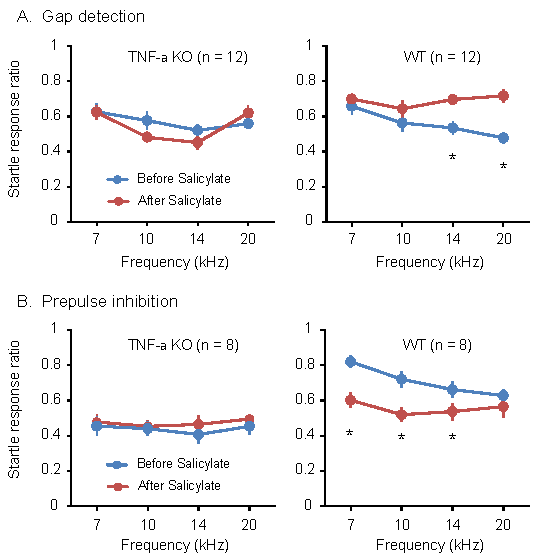
\includegraphics[width=4in]{images/C4F2}}

\begin{changemargin}{1in}{1in}
\footnotesize{Figure 2.}
\end{changemargin}

\subsection{Cortical infusion of recombinant TNF-\textalpha{} results in tinnitus}

To test whether TNF-\textalpha{} is sufficient to cause tinnitus symptoms, we infused mouse recombinant TNF-\textalpha{} into the right hemisphere auditory cortex of normal-hearing WT and TNF-\textalpha{} KO mice. Control WT and KO mice were infused with carrier solution containing artificial cerebrospinal fluid and mouse albumin. Gap detection and PPI performance was examined in three daily sessions prior to the injection and only the third session was used as the baseline performance. Mice were tested again after 3 days of post-surgical recovery. Gap detection performance was analyzed with a 4-way ANOVA on genotype (WT vs. KO), treatment (before vs. after infusion), drug (TNF-\textalpha{} vs. albumin) and frequency of the background tone. There were main effects of treatment ($F_{1,152}=8.619$, $p=0.0038$) and drug ($F_{1,152}=4.476$, $p=0.032$). There was also treatment x drug interaction ($F_{1,152}=5.730$, $p=0.018$), indicating that TNF-\textalpha{} and albumin changed gap detection performance differently. However, the interaction was independent of genotype (treatment x drug x genotype interaction, $F_{1,152}=0.007$, $p=0.94$) suggesting that TNF-\textalpha{} infusion had similar effects on both WT and KO mice. Posthoc t-test indicates that TNF-\textalpha{} significantly impaired gap detection at 20 kHz (WT: t12 = 4.19, $p=0.0013$; KO: t12 = 2.45, $p=0.035$), but not at other frequencies.

A similar 4-way ANOVA on PPI failed to show significant treatment x drug interaction ($F_{1,152}=0.391$, $p=0.53$) indicating that TNF-\textalpha{} did not alter PPI performance (Figure 3).

\centerline{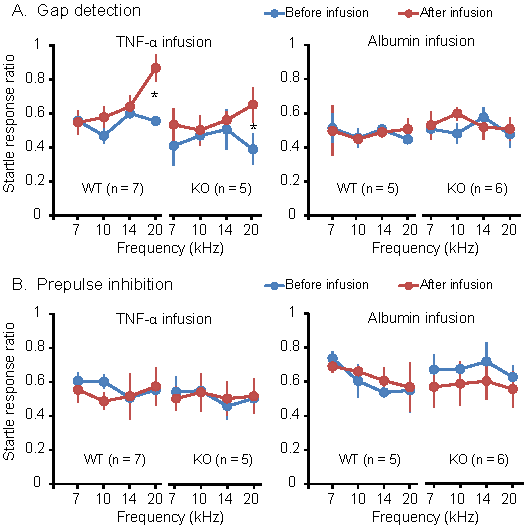
\includegraphics[width=4in]{images/C4F3}}

\begin{changemargin}{1in}{1in}
\footnotesize{Figure 3. TNF-\textalpha{} is sufficient to cause tinnitus. (A) Auditory cortical infusion of mouse recombinant TNF-\textalpha{} results in behavioral signs of tinnitus both WT and TNF-\textalpha{} KO mice, as indicated by impaired gap detection performance. Infusion of mouse albumin did not result in tinnitus. (B) Prepulse inhibition was not altered by infusion of TNF-\textalpha{} or albumin. *$p<0.05$.}
\end{changemargin}

\subsection{Hearing loss-induced downregulation of GAD65 expression was reduced in TNF-\textalpha{} KO mice}

\subsection{Plasticity of ipsilateral inputs following contralateral hearing lesion is impaired in TNF-\textalpha{} KO mice}

To examine the electrophysiological changes in primary auditory cortex following unilateral NIHL, we independently stimulated the lesioned and intact ear while recording multi-unit activity from auditory cortex contralateral to the lesioned ear. Na\"ive WT and KO animals displayed strong, tonotopically-organized RFs in response to contralateral stimulation (Figure 4). As reported previously (\cite{Yang2013}), evoked firing rates are lower in KO animals (WT-Left-na\"ive vs KO-Left-na\"ive, $p=0.0190$, Tukey’s HSD). Unilateral NIHL led to a drastic reduction in the proportion of units responsive to the lesioned ear in both genotypes, however only in WT mice did NIHL result in a significant increase in the proportion of units responsive to the spared ear in ipsilateral cortex (Na\"ive vs NIHL, WT-Left: $p<<0.001$, KO-Left: $p=0.0011$, WT-Right: $p=0.012$, KO-Right: $p=0.999$, Tukey’s HSD, Figure 5A). The mean evoked firing rate and RF size showed similar patterns of changes following NIHL, i.e., decreases in both genotypes for contralateral stimulation, and increases only in WT animals for ipsilateral stimulation (Na\"ive vs NIHL, mean evoked firing rate: WT-Left: $p<<0.001$, KO-Left: $p=0.166$, WT-Right: $p=0.045$, KO-Right: $p=1.00$, Figure 5B; RF size: WT-Left: $p<<0.001$, KO-Left: $p=0.0170$, WT-Right: $p=0.007$, KO-Right: $p=0.999$, Tukey’s HSD; Figure 5C). One exception was that in KO animals the decrease in mean firing rate for contralateral stimulation post-NIHL was a trend that did not reach significance.

\centerline{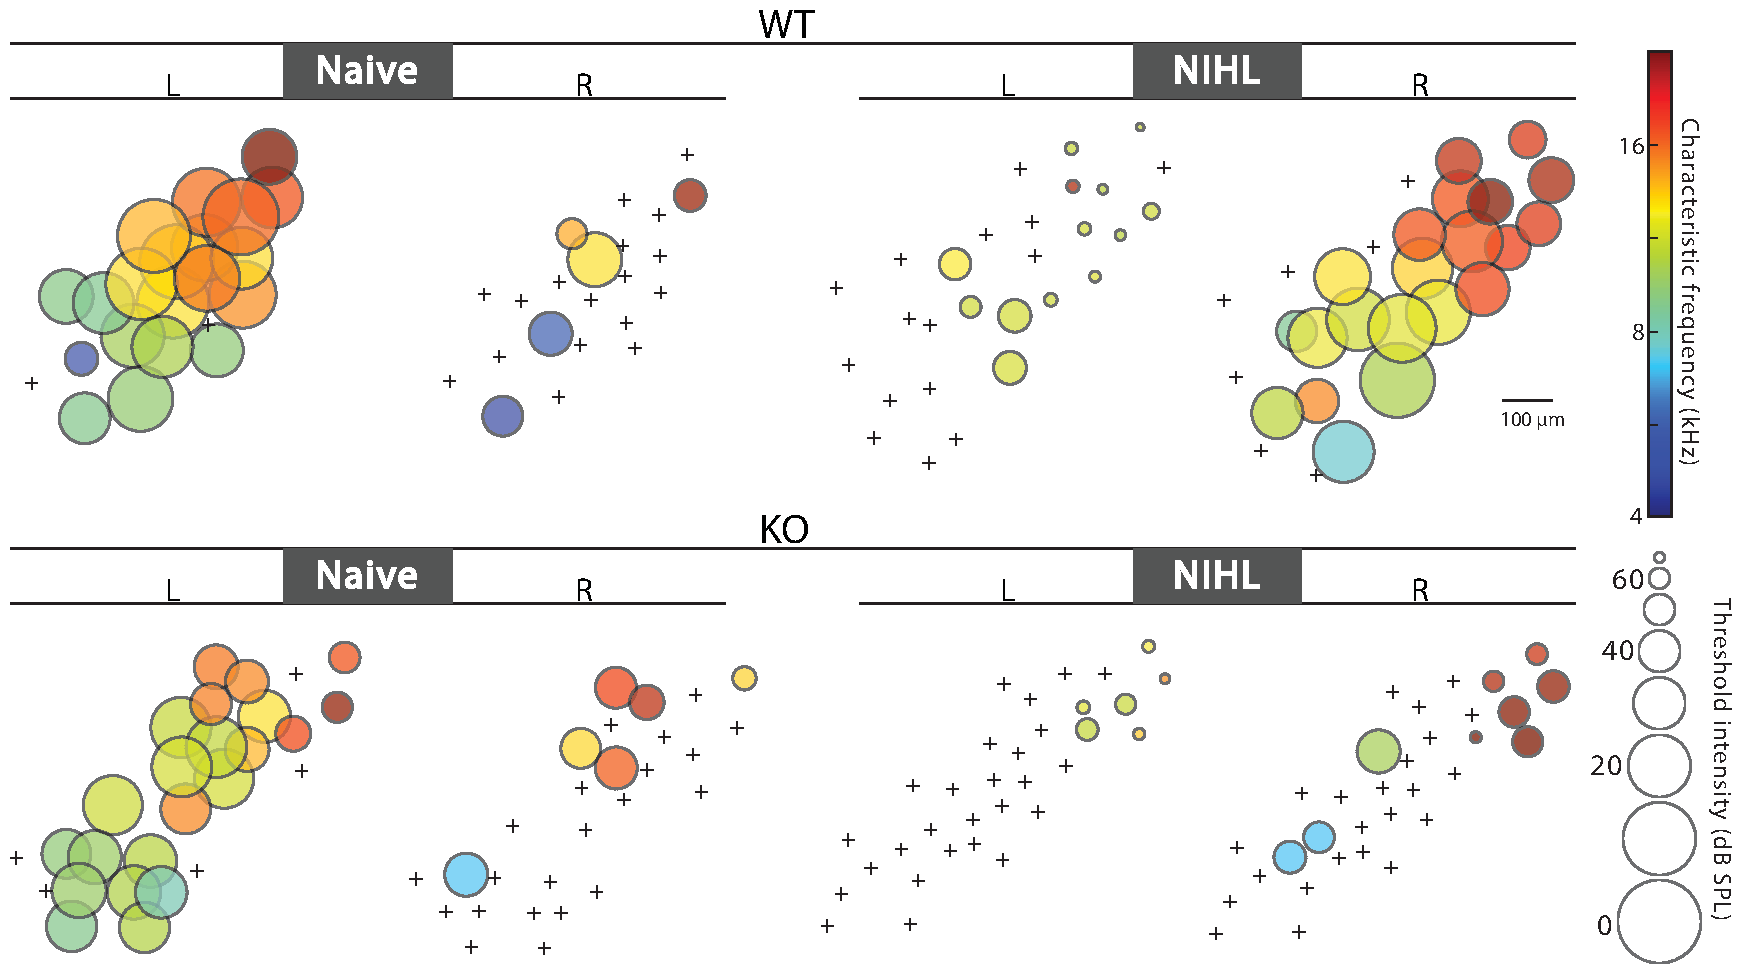
\includegraphics[width=4in]{images/C4F4}}

\begin{changemargin}{1in}{1in}
\footnotesize{Figure 4. Example contralateral (L) and ipsilateral (R) maps for WT and KO in naïve and NIHL animals. Each circle represents the multi-unit recording from one site, with characteristic frequency and threshold intensity represented by color and radius, respectively. Unresponsive sites are marked by a +. In naïve WT and KO animals, contralateral maps in naïve animals have low thresholds and few non-responsive sites, while ipsilateral maps have few responsive sites. Contralateral responses are nearly eliminated following NIHL in WT and KO, however only WT animals show strong augmentation of the ipsilateral map.}
\end{changemargin}

\printbibliography

\chapter{Discussion}

\section{Genetic Knockout Models and Critical Period Plasticity}

In the present work, I examined the critical period for plasticity in two genetic knockout models, \textit{Fmr1} KO and TNF-\textalpha{} KO. I sought to understand the link between genes, specific plasticity mechanisms, plasticity of larger-scale networks, and perception.

% Intro
In Chapters 2 and 3, I described auditory map development in mice lacking \textit{Fmr1} and TNF-\textalpha{}, respectively. Here, I will attempt to put these findings into the context of our current understanding of cortical critical periods with specific attention to how the results fit into the growing body of evidence showing the importance of inhibition in critical period expression. In Chapter 4, I turn to the auditory disorder tinnitus, which I hypothesize results from maladaptive homeostatic plasticity.

% In the auditory cortex, the earliest critical period is that for the allocation of cortical area to different sound frequencies. This has been best studied in rats, where it was found to take place between post-natal day 11 (P11) and P14 (\cite{DeVillers-Sidani2008}). During this period, simply rearing in the presence of a pure tone can dramatically and permanently increase the cortical area tuned to the exposed tone and can affect perception long into adulthood (\cite{Han2007}). The studies in the current work largely pertain to this critical period, although it should be noted that subsequently, auditory cortex undergoes critical periods for more complex sound features, such as sweep direction and binaural cues (\cite{Insanally2009, Popescu2010a}).

\subsection{Inhibition and Critical Periods}
% inhibition is important, Fagiolini 2000 study
The precise mechanism underlying the expression of critical periods has long remained a mystery, although recent work has revealed that the maturation of inhibitory circuits plays a crucial role. Some evidence for the importance of inhibition comes from experiments that have prematurely opened or that delayed the critical period for ocular dominance plasticity. In wild-type mice, depriving vision from one eye early in life causes a drastic remapping of visual cortex to respond to the open eye, whereas similar monocular deprivation later in life has no lasting effect. In mice lacking \textit{Gad65}, one of two enzymes responsible for synthesizing the inhibitory neurotransmitter GABA, monocular deprivation is unable to cause ocular dominance shifts at any age, indicating that the gene is necessary for critical period expression (\cite{Fagiolini2000}). Importantly, supplementing inhibition with benzodiazepine GABA$_\mathrm{A}$ agonists immediately initiates the critical period in \textit{Gad65} KO mice, even much later in life. Furthermore, the same benzodiazepam treatment leads to precocious critical period in wild-type mice (\cite{Fagiolini2000}). Another study using a mouse line with elevated levels of brain-derived neurotrophic factor (BDNF), which accelerates maturation of inhibitory neurons, found that the critical period for ocular dominance is also accelerated (\cite{Hanover1999, Huang1999}). These studies suggest that critical period learning is permitted when inhibitory tone passes a particular threshold level.

% Fagiolini 2004, parvalbumin-positive cells are important
Inhibitory neurons are not a homogeneous class of cells but rather come in a variety of different types, which presumably perform different roles in the brain. Across multiple studies, the fast-spiking parvalbumin-positive interneurons appear to play a crucial role in critical period expression. These neurons synapse on the soma of pyramidal cells where they provide rapid feed-forward and feed-back inhibition (\cite{Markram2004}). Building off of the previously mentioned finding that pharmacological activation of GABA$_\mathrm{A}$ receptors leads to a precocious critical period, experimenters took advantage of genetic ``knock-in" mouse lines in which GABA$_\mathrm{A}$ receptors containing certain subunits are rendered insensitive to diazepam to selectively activate putative subpopulations of inhibitory neurons. Different classes of inhibitory neurons make contact at synapses enriched for GABA$_\mathrm{A}$ receptors containing particular subunits, e.g. GABA$_\mathrm{A}$ receptors containing \textalpha{}1 subunits are preferentially located on the soma post-synaptic to parvalbumin-positive inhibitory neurons (\cite{Fagiolini2004}). This additional information enabled the experiment to address whether critical period expression requires activity in a particular class of inhibitory neurons versus inhibition in general.  Premature initiation of the critical period is only possible when \textalpha{}1 subunit-containing GABA$_\mathrm{A}$ receptors are activated, suggesting that parvalbumin-positive networks play an important role in the critical period.

% studies of circuits in auditory cortex
Inhibitory neurons appear to be important for critical periods in the auditory cortex as well. In fact a more detailed understanding of the role of inhibition comes from experiments that measure inhibitory and excitatory currents in the auditory cortex before, during, and after the critical period. In the adult auditory cortex, the frequency-intensity tuning of excitation and inhibition are precisely matched, i.e. transient auditory stimuli elicit a consistent pattern of excitation followed by rapid co-tuned inhibition (\cite{Wehr2003, Wehr2005}). Before the critical period for map plasticity, inhibitory circuits are not co-tuned and are not activated with such temporal precision, but after brief exposure to patterned sound stimuli, excitation and inhibition become co-tuned and resistant to further changes, bearing greater resemblance to the adult circuit (\cite{Dorrn2010}).

% Exposure to broadband noise prevents the normal maturation of parvalbumin-positive interneurons.
Even more convincing evidence comes from the discovery that noise exposure causes cortical networks to undergo a reversal of inhibitory circuit maturation marked by reduced GABA$_\mathrm{A}$-\textalpha{}1 and \textbeta{}2/3 subunits and reduced BDNF levels, which as already mentioned are important in the development of inhibitory circuits. Functional indicators of maturational state are also altered, including the re\"emergence of broad excitatory receptive fields, poor following of temporally modulated sounds, and decreased neural synchrony. Importantly, following cessation of noise exposure, cortex in these animals regains the ability to undergo pure-tone evoked map expansion (\cite{Zhou2011}).

\subsection{\textit{Fmr1} and Critical Periods}
Given the wealth of evidence that development of inhibitory circuits is important for expression of a critical period, it is important to interpret the results of the current work in terms of effects on inhibition. In Chapter 2, I presented results that indicate the critical period for auditory map plasticity is impaired in mice lacking \textit{Fmr1}. Other studies in this model organism confirm that they indeed show signs of altered inhibition, or more specifically, disrupted excitatory-inhibitory balance (\cite{Gibson2008}). Perhaps the most salient indication of malfunctioning inhibition in Fragile X syndrome is the increased susceptibility to audiogenic seizures, both in human patients and in animal models (\cite{Hagerman, Chen2001}). This observation led to many studies finding weakened inhibition in FXS, although given the more recent observation of links between inhibition and critical periods, the results can be interpreted more broadly in terms of early learning and circuit formation (\cite{ElIdrissi2005}). Overall protein levels of GABA$_\mathrm{A}$ receptor \textalpha{}1, \textbeta{}2, and \textdelta{} subunits are reduced in \textit{Fmr1} KO forebrain, as well as important enzymes related to GABA metabolism, GABA transaminase and succinic semialdehyde dehydrogenase (\cite{Adusei2010}). As mentioned previously, the \textalpha{}1 subunit is necessary for expression of the critical period for ocular dominance, so if we generalize the finding to auditory cortex, it could contribute to our observed critical period impairment. Consistent with ocular dominance plasticity studies implicating parvalbumin-positive associated \textalpha{}1-containing GABA$_\mathrm{A}$ receptors, \textit{Fmr1} KO mice display a 20\% reduction in the density of parvalbumin-positive neurons in neocortex, while they show no significant decrease in other inhibitory subtypes, including calbindin- and calretinin-positive neurons (\cite{Selby2007}).

\subsection{TNF-\textalpha{} and Critical Periods}

I took advantage of the TNF-\textalpha{} KO mouse line, in which homeostatic plasticity is disrupted, to study the role of homeostatic plasticity in two markedly different phenomena: the critical period for map plasticity and tinnitus.
% As mentioned previously, the neonatal auditory cortex is distinct from the adult brain in many ways, including having weaker inhibition and ungated LTP.
The benefit of studying the same process at different stages of brain development is that we can gain an understanding of how the role and operation of that process changes in response to different exogenous conditions. In my research, I examined homeostatic plasticity in the face of multiple stimulation contexts and at two stages of brain development. The conditions can be summarized as: 1. early-life exposure to normal ambient auditory stimuli (Chapter 3), 2. early-life exposure to single-tone pip trains (Chapter 3), 3. early-life exposure to multi-tone pip trains (Chapter 3), and 4. adult hearing loss (Chapter 4). As mentioned before, there are multiple forms of homeostatic plasticity, including forms that do not appear to involve TNF-\textalpha{} (\cite{Stellwagen2006}). From here, unless otherwise specified, I will reserve ``homeostatic plasticity" to refer to those homeostatic mechanisms depending on TNF-\textalpha{}.

In Chapter 3, I presented data that show how the absence of TNF-\textalpha{} impairs auditory cortical development in a normal sound environment while pure-tone evoked auditory map expansion is intact. There are many steps that give rise to the tonotopic map. In mice, precise tonotopy develops before hearing onset, and depends on patterned spontaneous calcium spikes generated in the spiral ganglia and driven by cholinergic cells in the medial olive (\cite{Elgoyhen1994, Cao2008, Clause2014}). Later, experience-driven refinements of the map occur (\cite{DeVillers-Sidani2008, Han2007}). It is not yet clear which of these stages relies on TNF-\textalpha{} since the knockout animals lack the protein throughout life. Exposure to single-tone pip trains begining at hearing onset normalized the frequency range to a degree. If we interpret the mechanism for this to be that tone exposure boosted cortical activity to within the homeostatic set range, eliminating the need for homeostatic plasticity (as explained later), it would indicate that  homeostatic plasticity during in the pre-hearing period is not strictly necessary for development of normal maps. This is fairly circuitous evidence, but it at least provides a clue to the true answer. Early auditory cortex mapping and temporal control of gene expression, for example using a Tet system (\cite{Gossen1995}), could reveal which time points require TNF-\textalpha{} expression. A future experiment could turn on TNF-\textalpha{} during development and off during the critical period. If such a manipulation led to normal maps, it would suggest that homeostatic plasticity is only needed during pre-hearing development.

Map development in standard mouse husbandry conditions was altered in TNF-\textalpha{} KO mice, which we found to have incomplete representations of the normal mouse hearing range. One could imagine that the ``standard" husbandry environment is an impoverished or unnatural sound milieu. Still, the important observation in our study is that in the same environment (regardless of whether or not it can be characterized as impoverished), WT animals develop maps that represent the full range of frequencies, with ordered tonotopy, in clear contrast to KO mice. Even if we accept that there is less sound energy in the husbandry environment, it only highlights the importance of homeostatic plasticity in normal map development. In the wild, it is reasonable to assume that average sound energy experienced by different animals and litters varies considerably, making mechanisms like TNF-\textalpha{}-dependent homeostatic plasticity critically important for their ability to regulate activity to a level permissive of normal map development.

In contrast, early-life exposure to single-tone pip trains did not depend on homeostatic plasticity, as indicated by the fact that exposure led to expansion of the area representing the exposure frequency in KO mice. In addition, even though the exposure consisted of a single frequency (25 kHz), it expanded the range of frequencies represented in individual KO maps compared to those in unexposed KO mice (Chapter 3, Figure 3). There are a few possibilities for how narrow-band stimulation might have affected this global map characteristic. Auditory cortical neurons respond to a broad range of frequencies. In our study, the average tuning bandwidth was $2.7\pm0.2$ octaves, and in the developing brain bandwidths are generally even larger (\cite{Zhang2001}). Using the conservative average value from our study, a neuron tuned to 9.8 kHz could still have been significantly activated by the exposure stimulus during development. In addition to this fact, map expansion was concurrently taking place, meaning that an even greater area of auditory cortex was activated by the exposure stimulus. This suggests the possibility that abnormally low activity levels in the KO brain prevented normal map development. Indeed, spontaneous and evoked firing rates were lower in KO animals than WT animals (Chapter 3, Figure 4F \& G). In this scenario, the pure-tone stimulus drove activity across a wide swath of cortex, and the elevated activity was sufficient to bring about development of the normal tonotopy. In this stimulus regime, homeostatic plasticity was unnecessary since stimulus conceivably boosted activity across auditory cortex.

Combining the \textit{Fmr1} and TNF-\textalpha{} studies gives us a clearer picture of how Hebbian and homeostatic mechanisms might interact to allow the critical period for auditory plasticity unfold. In an auditory environment enriched with a pure-tone, neurons with some preference for that tone will over the course of exposure be repeatedly driven by that stimulus. This could engage Hebbian mechanisms to strengthen synapses activated by the exposed frequency and re-tune the neurons, leading to a macroscopic map expansion. This hypothesis is consistent with the absence of map expansion in \textit{Fmr1} KO mice, which lack the ability to undergo cortical LTP. It also is in line with the finding that in TNF-\textalpha{} KO mice, which are deficient in homeostatic plasticity but possess the ability to undergo cortical LTP, map expansion progresses normally. As discussed previously, LTP is likely to be a key plasticity mechanism in the critical period for auditory map plasticity as its ability to be induced at thalamocortical synapses is correlated with the timing of the critical period (\cite{Chun2013}). The picture is complicated by the fact that MPEP is able to restore auditory map plasticity, but does not restore cortical LTP (\cite{Wilson2007}). One possibility is that the conflicting results reflect a difference in \textit{in vivo} and \textit{in vitro} experimental methods---in our study, MPEP was administered for many days over the course of sound exposure, whereas in a slice preparation the drug is applied for a relatively short time.

A clear \textit{in vivo} realization of theoretical principles of plasticity comes from the broadband stimuluation regime of the enriched environment (EE), in which neurons have to contend with competition from multiple strong inputs. A simple plasticity model governed by LTP would predict that strong repeated stimulation would trigger LTP and strengthen inputs from a wide range of frequencies, leading to increased receptive field bandwidths. In fact, only in KO animals do bandwidths increase, whereas in WT animals bandwidths actually decrease. The KO condition stands as a clear example of the problem of LTP in the absence of homeostatic plasticity in which positive-feedback leads to synapse strengthening towards saturation. In WT mice, the homeostatic mechanism of synaptic scaling decreases the engagement of LTP for more weakly associated inputs while still allowing LTP for inputs that strongly drive the neuron. Together, LTP and homeostatic plasticity produce a system in which competition between inputs can lead to refinement of selectivity, which is important for perceptual discrimination of stimuli (\cite{Han2007}).

\section{Tinnitus and plasticity}

Critical period learning is but one of the many phenomena brought about by neural plasticity. The brain is plastic throughout life, and as I discussed previously, adult plasticity shares many of the specific cellular and molecular mechanisms that underlie critical period learning. We generally think of plasticity as a desirable trait for a neural network to possess---the ability to incorporate past experiences into future decisions can confer significant survival and reproduction advantages on an organism. However, the immense power plasticity wields over brain function can under certain circumstances lead to undesired consequences. ``Maladaptive plasticity" is simply any plasticity that results in impaired brain function, and is thought to be involved in phantom perception following limb amputation, motor remapping after a stroke, and, as I demonstrate in Chapter 4, tinnitus following hearing loss (\cite{Flor2006, Takeuchi2012}).

% One motivating question in my research was how the changes to neural circuits experienced in tinnitus are related to normal plasticity mechanisms. Does tinnitus result from a distinct pathological plasticity mechanism that is triggered by the loss of normal sensory input or does it result from the subversion of typically advantageous plasticity mechanisms driven by abnormal signals from the damaged cochlea? If it is the latter, it is important to understand the interplay between the cellular and molecular mechanisms of plasticity and the neural signals on which they operate.

\section{Conclusion}
For practical reasons, experimental manipulations usually focus on increasing or decreasing levels of meone protein. This is the paradigm used in all of the individual experiments used in this study. If one draws conclusions from the converging results of many single manipulations, it is possible to come up with plausible models for how the brain is actually operating. However, it is important to keep in mind that, however pragmatic it might be to partition biological systems into individual components, biological systems are highly interconnected.
...

% For example, in my interpretation of my critical period studies, I drew heavily on the current theory that inhibitory tone is a key determinant of the ability of cortex to undergo critical period learning. Still, despite a large body of evidence showing that inhibition is important, there is still no clear mechanism for how immature inhibitory networks allow critical period expression. One possibility is that weakened inhibition simply permits elevated activity levels that are favorable to Hebbian activity-dependent plasticity. One study suggests that a mutant line with enhanced inhibition also loses the ability to undergo LTP in the dentate gyrus. Tamping down inhibition using bicuculine, a GABA$_\mathrm{A}$ receptor antagonist restored the ability to undergo LTP, and in addition, LTP could be blocked in wild-type mice by administration of diazepam, a GABA$_\mathrm{A}$ receptor agonist (\cite{Levkovitz1999}). In auditory cortex, there also seems to be a link between disinhibition and LTP. While LTP of thalamocortical synapses is readily elicited in neonates during the critical period, the same protocol fails to elicit LTP in adults. However, removing inhibitory currents using intracellular injection of picrotoxin in cortical pyramidal neurons or induction of LTD at inhibitory synapses rendered the thalamocortical synapses capable of undergoing LTP. Group I metabolic glutamate receptors appeared to underlie this plasticity since MPEP prevented the induction of LTP even with reduced inhibition (\cite{Chun2013}). Studies like show the importance of considering how the many uniquely identified conceptual elements of the brain are interrelated, and future studies stand to make significant progress by considering how different processes interact.

\printbibliography

\end{document}
